\documentclass[9pt, letterpaper, landscape]{article}
\usepackage[utf8]{inputenc}
\usepackage[T1]{fontenc}
\usepackage[margin=0.3in, top=0.5in, bottom=0.4in]{geometry}
\usepackage{amsmath, amssymb, bm, amsthm}
\usepackage{tikz}
\usetikzlibrary{calc, shapes.geometric, shadows.blur, positioning, arrows.meta, matrix, decorations.pathreplacing}
\usepackage[most]{tcolorbox}
\usepackage{multicol}
\usepackage{ebgaramond} 
\usepackage{titlesec}
\usepackage{fancyhdr}
\usepackage{tabularx}
\usepackage{booktabs}

% --- PALETA CROMÁTICA "ECONOMÍA MATEMÁTICA 2025" ---
\definecolor{VogueBlack}{RGB}{10, 10, 10}      
\definecolor{MITCrimson}{RGB}{163, 31, 52}     
\definecolor{GoldLeaf}{RGB}{170, 145, 90}      
\definecolor{SlateGrey}{RGB}{60, 65, 75}       
\definecolor{SoftLinen}{RGB}{253, 252, 250}    
\pagecolor{SoftLinen}


\titleformat{\section}{\color{VogueBlack}\normalfont\Large\scshape\centering}{}{0em}{#1}[\vspace{2pt}\rule{0.3\textwidth}{0.5pt}]
\titleformat{\subsection}{\color{SlateGrey}\normalfont\large\scshape}{}{0em}{#1}

% --- CAJAS EDITORIALES ---
\tcbset{
    voguebox/.style={
        enhanced, sharp corners, boxrule=0pt,
        colback=white, colframe=VogueBlack,
        borderline north={1.5pt}{0pt}{VogueBlack},
        borderline south={0.3pt}{0pt}{GoldLeaf},
        drop shadow={black!5},
        fonttitle=\bfseries\scshape\small,
        coltitle=VogueBlack,
        attach boxed title to top left={xshift=0mm, yshift=-2.5mm},
        boxed title style={colback=white, boxrule=0pt}
    },
    definitionbox/.style={
        voguebox,
        borderline north={1.5pt}{0pt}{MITCrimson},
    },
    theorembox/.style={
        voguebox,
        borderline north={1.5pt}{0pt}{GoldLeaf},
    }
}

% --- CREAR LOS ENTORNOS DE CAJA (FALTA ESTO) ---
\newtcolorbox{voguebox}[1][]{voguebox,#1}
\newtcolorbox{definitionbox}[1][]{definitionbox,#1}
\newtcolorbox{theorembox}[1][]{theorembox,#1}

% --- COMANDOS PERSONALIZADOS ---
\newcommand{\secbar}{\begin{center}
\begin{tikzpicture}\draw[GoldLeaf, line width=1.5pt] (0,0) -- (4,0);\end{tikzpicture}\end{center}}

\begin{document}

% --- CABECERA PRINCIPAL ---
\begin{tikzpicture}[remember picture, overlay]
    \fill[VogueBlack] ($(current page.north west)$) rectangle ($(current page.north east) + (0,-0.3in)$);
    \node[white, anchor=west] at ($(current page.north west) + (0.5in, -0.15in)$) {\fontfamily{phv}\selectfont \textbf{ECONOMÍA MATEMÁTICA UPTC}};
    \node[white, anchor=east] at ($(current page.north east) + (-0.5in, -0.15in)$) {\textsc{\small Capítulo 4 // Diciembre 2025}};
\end{tikzpicture}

\begin{center}
    \vspace*{10pt}
    {\fontsize{48}{52}\selectfont\textbf{Modelos Lineales}} \\
    \vspace{4pt}
    {\fontsize{36}{40}\selectfont\textbf{\&\ Álgebra de Matrices}} \\
    \vspace{4pt}
    {\large\textsc{Fundamentos de Economía Matemática}} \\
    \vspace{8pt}
    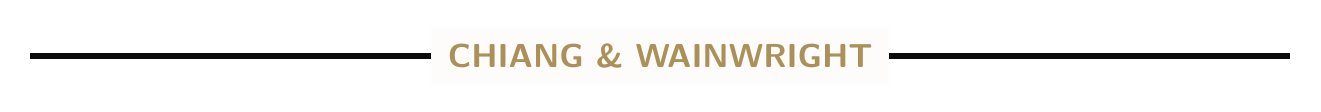
\begin{tikzpicture}
        \draw[line width=2pt, VogueBlack] (0,0) -- (16,0);
        \node[fill=SoftLinen, inner sep=6pt, text=GoldLeaf] at (8,0) {\large\textsf{\textbf{CHIANG \& WAINWRIGHT}}};
    \end{tikzpicture}
\end{center}

\begin{multicols*}{3}

% ========================================
% SECCIÓN 1: INTRODUCCIÓN Y CONTEXTO
% ========================================

\section{I. Introducción al Álgebra Matricial}

\noindent\textbf{EL DESAFÍO DIMENSIONAL.} En economía matemática, el análisis de modelos con múltiples variables requiere metodologías que vayan más allá de las técnicas escalares tradicionales. El \textbf{álgebra de matrices} emerge como la herramienta fundamental para abordar el análisis estático o de equilibrio cuando el número de variables es grande.

\begin{definitionbox}\textbf{Necesidad del Álgebra Matricial}
\small Cuando un modelo de mercado aumenta de uno a dos o más artículos, las fórmulas de eliminación de variables se vuelven rápidamente inmanejables. El álgebra de matrices proporciona una solución sistemática y elegante a este problema de complejidad.
\end{definitionbox}

\subsection{Ventajas Cruciales}

El álgebra de matrices ofrece tres ventajas fundamentales para el análisis económico:

\begin{enumerate}
    \item \textbf{Compacidad Notacional}: Proporciona una forma compacta de escribir sistemas de ecuaciones, incluso muy grandes.
    \item \textbf{Teoría de Existencia}: Permite probar la existencia de soluciones mediante la evaluación de determinantes.
    \item \textbf{Método Sistemático}: Suministra un procedimiento algorítmico para encontrar soluciones cuando existen.
\end{enumerate}

\subsection{Linealidad y Transformaciones}

\begin{voguebox}\textbf{Restricción de Linealidad}
\small El álgebra de matrices se aplica específicamente a \textbf{sistemas de ecuaciones lineales}. Sin embargo, esta restricción no es limitante: modelos no lineales pueden transformarse mediante cambios de variables (logaritmos, etc.) en relaciones lineales equivalentes.
\end{voguebox}

\noindent\textbf{Ejemplo de Transformación:}
\begin{equation}
y = ax^b \quad \xrightarrow{\log} \quad \log y = \log a + b\log x
\end{equation}

% ========================================
% SECCIÓN 2: MATRICES Y VECTORES
% ========================================

\section{II. Matrices como Arreglos Rectangulares}

\noindent\textbf{LA ESTRUCTURA FUNDAMENTAL.} Una matriz es un \textbf{arreglo rectangular de números, parámetros o variables}, organizados en filas (renglones) y columnas. Los elementos individuales se identifican mediante subíndices dobles.

\subsection{Definición Formal}

\begin{definitionbox}[title=Matriz]
\small Una matriz $\mathbf{A}$ de dimensión $m \times n$ es un arreglo rectangular de $m$ filas y $n$ columnas:
\begin{equation}
\mathbf{A} = \begin{bmatrix}
a_{11} & a_{12} & \cdots & a_{1n} \\
a_{21} & a_{22} & \cdots & a_{2n} \\
\vdots & \vdots & \ddots & \vdots \\
a_{m1} & a_{m2} & \cdots & a_{mn}
\end{bmatrix}
\end{equation}
Donde $a_{ij}$ denota el elemento en la fila $i$ y columna $j$.
\end{definitionbox}

\subsection{Representación de Sistemas Lineales}

Para un sistema de $m$ ecuaciones lineales en $n$ variables, utilizamos tres configuraciones rectangulares:

\begin{itemize}
    \item $\mathbf{A}$: Matriz de coeficientes $(m \times n)$
    
    \item $\mathbf{x}$: Vector de variables $(n \times 1)$
    \item $\mathbf{d}$: Vector de términos constantes $(m \times 1)$
\end{itemize}

\noindent El sistema completo se representa como: $\mathbf{Ax} = \mathbf{d}$


\subsection{Visualización Matricial}

\begin{center}
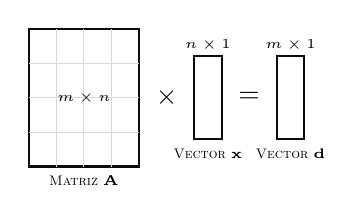
\begin{tikzpicture}[scale=0.7]
    % Matriz A
    \draw[VogueBlack, thick] (0,0) rectangle (2,2.5);
    \draw[SlateGrey!20] (0.5,0) -- (0.5,2.5);
    \draw[SlateGrey!20] (1,0) -- (1,2.5);
    \draw[SlateGrey!20] (1.5,0) -- (1.5,2.5);
    \draw[SlateGrey!20] (0,0.625) -- (2,0.625);
    \draw[SlateGrey!20] (0,1.25) -- (2,1.25);
    \draw[SlateGrey!20] (0,1.875) -- (2,1.875);
    \node[below, font=\tiny\scshape] at (1,0) {Matriz $\mathbf{A}$};
    \node at (1,1.25) {\tiny $m \times n$};
    
    % Símbolo multiplicación
    \node at (2.5, 1.25) {$\times$};
    
    % Vector x
    \draw[VogueBlack, thick] (3,0.5) rectangle (3.5,2);
    \node[below, font=\tiny\scshape] at (3.25,0.5) {Vector $\mathbf{x}$};
    \node at (3.25,2.2) {\tiny $n \times 1$};
    
    % Símbolo igual
    \node at (4, 1.25) {$=$};
    
    % Vector d
    \draw[VogueBlack, thick] (4.5,0.5) rectangle (5,2);
    \node[below, font=\tiny\scshape] at (4.75,0.5) {Vector $\mathbf{d}$};
    \node at (4.75,2.2) {\tiny $m \times 1$};
\end{tikzpicture}
\end{center}

% ========================================
% SECCIÓN 3: VECTORES COMO MATRICES ESPECIALES
% ========================================

\section{III. Vectores como Matrices Especiales}

\noindent\textbf{LA DUALIDAD VECTORIAL.} Un vector es una matriz que posee una única columna o un único renglón, representando casos especiales de dimensiones matriciales.

\subsection{Tipos de Vectores}

\begin{theorembox}\textbf{Clasificación Vectorial}
\small
\textbf{1. Vector Columna} ($m \times 1$):
\begin{equation}
\mathbf{x} = \begin{bmatrix} x_1 \\ x_2 \\ \vdots \\ x_m \end{bmatrix}
\end{equation}

\textbf{2. Vector Renglón} ($1 \times n$):
\begin{equation}
\mathbf{x}' = \begin{bmatrix} x_1 & x_2 & \cdots & x_n \end{bmatrix}
\end{equation}
\end{theorembox}

\subsection{Notación y Convenciones}

\begin{itemize}
    \item El apóstrofo ($'$) o superíndice $T$ denota la \textbf{transpuesta}
    \item $\mathbf{x}'$ representa un vector renglón
    \item $\mathbf{x}$ sin notación adicional típicamente denota vector columna
\end{itemize}

\subsection{Interpretación Geométrica}

\begin{voguebox}\textbf{Espacio Vectorial}
\small Todo vector con $n$ componentes puede interpretarse como una \textbf{$n$-tupla ordenada}, equivalente a un punto en un espacio de dimensión $n$: $\mathbb{R}^n$.
\end{voguebox}



% ========================================
% SECCIÓN 4: OPERACIONES CON MATRICES
% ========================================

\section{IV. Operaciones Fundamentales}

\noindent\textbf{LA ARITMÉTICA MATRICIAL.} Las operaciones con matrices siguen reglas algebraicas específicas que difieren del álgebra escalar tradicional.

\subsection{1. Igualdad de Matrices}

\begin{definitionbox}\textbf{Igualdad Matricial}
\small Dos matrices $\mathbf{A} = [a_{ij}]$ y $\mathbf{B} = [b_{ij}]$ son iguales si y solo si:
\begin{enumerate}
    \item Poseen la misma dimensión: $m \times n$
    \item Todos los elementos correspondientes son idénticos: $a_{ij} = b_{ij}$ para todo $i, j$
\end{enumerate}
\end{definitionbox}

\subsection{2. Suma y Resta de Matrices}

\noindent\textbf{Condición de Conformabilidad:} Las matrices deben tener la \textbf{misma dimensión}.

\begin{equation}
\mathbf{C} = \mathbf{A} + \mathbf{B} \implies c_{ij} = a_{ij} + b_{ij}
\end{equation}

\noindent\textbf{Ejemplo Numérico:}
\begin{equation}
\begin{bmatrix} 4 & 9 \\ 2 & 1 \end{bmatrix} + \begin{bmatrix} 2 & 0 \\ 0 & 7 \end{bmatrix} = \begin{bmatrix} 6 & 9 \\ 2 & 8 \end{bmatrix}
\end{equation}

\subsection{3. Multiplicación Escalar}

\begin{definitionbox}\textbf{Escalamiento Matricial}
\small Multiplicar una matriz por un escalar $\alpha$ implica multiplicar cada elemento:
\begin{equation}
\alpha\mathbf{A} = [\alpha a_{ij}]
\end{equation}
\end{definitionbox}

\noindent\textbf{Ejemplo:}
\begin{equation}
7\begin{bmatrix} 3 & -1 \\ 0 & 5 \end{bmatrix} = \begin{bmatrix} 21 & -7 \\ 0 & 35 \end{bmatrix}
\end{equation}

\subsection{Visualización de Operaciones}

\begin{center}
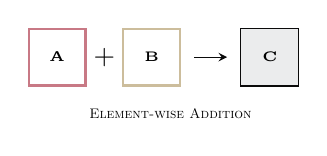
\begin{tikzpicture}[scale=0.6]
    % Suma
    \draw[MITCrimson!60, thick] (0,0) rectangle (1.2,1.2);
    \node at (0.6, 0.6) {\tiny $\mathbf{A}$};
    \node at (1.6, 0.6) {$+$};
    \draw[GoldLeaf!60, thick] (2,0) rectangle (3.2,1.2);
    \node at (2.6, 0.6) {\tiny $\mathbf{B}$};
    \draw[->, >=stealth, VogueBlack] (3.5,0.6) -- (4.2,0.6); % CAMBIADO: >=stealth
    \draw[VogueBlack, thick] (4.5,0) rectangle (5.7,1.2);
    \fill[SlateGrey!10] (4.5,0) rectangle (5.7,1.2);
    \node at (5.1, 0.6) {\tiny $\mathbf{C}$};
    \node[below, font=\tiny\scshape] at (3,-0.3) {Element-wise Addition};
\end{tikzpicture}
\end{center}

% prueba 
\section{V. Multiplicación de Matrices}

\noindent\textbf{LA OPERACIÓN FUNDAMENTAL.} La multiplicación de matrices es la operación más importante y compleja del álgebra matricial, fundamental para representar sistemas de ecuaciones lineales.

\subsection{Condición de Conformabilidad}

\begin{theorembox}\textbf{Regla Dimensional}
\small El producto $\mathbf{AB}$ está definido si y solo si:
\begin{equation}
\mathbf{A}_{m \times \colorbox{GoldLeaf!20}{$n$}} \times \mathbf{B}_{\colorbox{GoldLeaf!20}{$n$} \times q} = \mathbf{C}_{m \times q}
\end{equation}
El número de \textbf{columnas} de $\mathbf{A}$ debe igual al número de \textbf{filas} de $\mathbf{B}$.
\end{theorembox}

\subsection{Definición del Producto}

Cada elemento $c_{ij}$ de la matriz producto se define como el \textbf{producto interior} de la fila $i$ de $\mathbf{A}$ con la columna $j$ de $\mathbf{B}$:

\begin{equation}
c_{ij} = \sum_{k=1}^{n} a_{ik}b_{kj} = a_{i1}b_{1j} + a_{i2}b_{2j} + \cdots + a_{in}b_{nj}
\end{equation}

\subsection{Ejemplo Detallado}

\noindent\textbf{Sistema de Ecuaciones Lineales:}
\begin{equation}
\begin{bmatrix} 6 & 3 & 1 \\ 1 & 4 & -2 \\ 4 & -1 & 5 \end{bmatrix} \begin{bmatrix} x_1 \\ x_2 \\ x_3 \end{bmatrix} = \begin{bmatrix} 6x_1 + 3x_2 + x_3 \\ x_1 + 4x_2 - 2x_3 \\ 4x_1 - x_2 + 5x_3 \end{bmatrix}
\end{equation}

\subsection{Visualización del Proceso}

\begin{center}
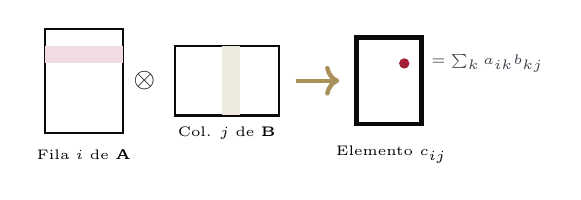
\begin{tikzpicture}[scale=0.55]
    % Matriz A
    \draw[VogueBlack, thick] (0,0) rectangle (1.8,2.4);
    \fill[MITCrimson!15] (0,1.6) rectangle (1.8,2);
    \node at (0.9,-0.5) {\tiny Fila $i$ de $\mathbf{A}$};
    
    % Símbolo
    \node at (2.3, 1.2) {$\otimes$};
    
    % Matriz B
    \draw[VogueBlack, thick] (3,0.4) rectangle (5.4,2);
    \fill[GoldLeaf!20] (4.1,0.4) rectangle (4.5,2);
    \node at (4.2, 0) {\tiny Col. $j$ de $\mathbf{B}$};
    
    % Flecha
    \draw[->, GoldLeaf, ultra thick] (5.8, 1.2) -- (6.8, 1.2);
    
    % Resultado
    \draw[VogueBlack, ultra thick] (7.2, 0.2) rectangle (8.7, 2.2);
    \filldraw[MITCrimson] (8.3, 1.6) circle (3pt);
    \node at (8, -0.5) {\tiny Elemento $c_{ij}$};
    
    \node[right, font=\tiny, SlateGrey] at (8.7, 1.6) {$= \sum_{k} a_{ik}b_{kj}$};
\end{tikzpicture}
\end{center}

\subsection{Propiedades Críticas}

\begin{voguebox}\textbf{No Conmutatividad}
\small En general: $\mathbf{AB} \neq \mathbf{BA}$

El orden de los factores \textbf{sí altera} el producto. Esta es la diferencia más importante respecto al álgebra escalar.
\end{voguebox}

\begin{theorembox}[title=Propiedad Asociativa]
\small La multiplicación de matrices es asociativa:
\begin{equation}
(\mathbf{AB})\mathbf{C} = \mathbf{A}(\mathbf{BC}) = \mathbf{ABC}
\end{equation}
(sujeto a conformabilidad dimensional)
\end{theorembox}



\subsection{5. La División: Una Operación Indefinida}

\begin{definitionbox}\textbf{Imposibilidad de la División}
\small \textbf{No es posible} dividir una matriz entre otra. La expresión $\mathbf{A}/\mathbf{B}$ carece de significado.

En su lugar, cuando existe la matriz inversa $\mathbf{B}^{-1}$, debemos especificar:
\begin{itemize}
    \item $\mathbf{AB}^{-1}$ (posmultiplicación por la inversa)
    \item $\mathbf{B}^{-1}\mathbf{A}$ (premultiplicación por la inversa)
\end{itemize}
\end{definitionbox}

\section{VI. Notación de Sumatoria ($\sum$)}

\noindent\textbf{LA ABREVIATURA COMPACTA.} La notación sigma es indispensable para expresar sumas largas de manera concisa.

\subsection{Estructura y Significado}

\begin{equation}
\sum_{j=1}^{n} x_j = x_1 + x_2 + \cdots + x_n
\end{equation}

\noindent\textbf{Componentes:}
\begin{itemize}
    \item $j$: Índice de sumatoria (toma valores enteros)
    \item $1$: Límite inferior
    \item $n$: Límite superior
    \item $x_j$: Sumando (función del índice)
\end{itemize}

\subsection{Aplicaciones en Álgebra Matricial}

\noindent\textbf{1. Funciones Polinomiales:}
\begin{equation}
\sum_{i=0}^{n} a_ix^i = a_0 + a_1x + a_2x^2 + \cdots + a_nx^n
\end{equation}

\noindent\textbf{2. Multiplicación de Matrices:}
\begin{equation}
c_{ij} = \sum_{k=1}^{n} a_{ik}b_{kj}
\end{equation}

\noindent El índice $k$ es un \textbf{índice simulado}: solo indica qué par de elementos se multiplica en cada término de la suma.

\subsection{Propiedades de la Sumatoria}

\begin{theorembox}\textbf{Leyes Distributivas}
\small
\begin{align}
\sum_{i=1}^{n} (a_i + b_i) &= \sum_{i=1}^{n} a_i + \sum_{i=1}^{n} b_i \\
\sum_{i=1}^{n} ca_i &= c\sum_{i=1}^{n} a_i
\end{align}
\end{theorembox}



\section{VII. Multiplicación de Vectores}

\noindent\textbf{CASOS ESPECIALES DEL PRODUCTO MATRICIAL.} La multiplicación de vectores produce resultados cualitativamente diferentes según el orden y la forma de los vectores.

\subsection{1. Vector Columna × Vector Renglón}

\noindent\textbf{Producto Exterior} ($\mathbf{uv}'$): Genera una \textbf{matriz}

\begin{equation}
\mathbf{u}_{m \times 1} \times \mathbf{v}'_{1 \times n} = \mathbf{M}_{m \times n}
\end{equation}

\noindent\textbf{Ejemplo:}
\begin{equation}
\begin{bmatrix} 3 \\ 2 \end{bmatrix} \begin{bmatrix} 1 & 4 & 5 \end{bmatrix} = \begin{bmatrix} 3 & 12 & 15 \\ 2 & 8 & 10 \end{bmatrix}
\end{equation}

\subsection{2. Vector Renglón × Vector Columna}

\noindent\textbf{Producto Interior} ($\mathbf{u}'\mathbf{v}$): Genera un \textbf{escalar}

\begin{equation}
\mathbf{u}'_{1 \times n} \times \mathbf{v}_{n \times 1} = s_{1 \times 1}
\end{equation}

\begin{definitionbox}\textbf{Producto Escalar}
\small
\begin{equation}
\mathbf{u} \cdot \mathbf{v} = \sum_{i=1}^{n} u_iv_i = u_1v_1 + u_2v_2 + \cdots + u_nv_n
\end{equation}
\end{definitionbox}

\noindent\textbf{Ejemplo:}
\begin{equation}
\begin{bmatrix} 3 & 4 \end{bmatrix} \begin{bmatrix} 9 \\ 7 \end{bmatrix} = 3(9) + 4(7) = 55
\end{equation}

\subsection{Aplicación Económica}

\begin{voguebox}\textbf{Costo Total de Compra}
\small Si $\mathbf{Q}'$ es un vector renglón de cantidades y $\mathbf{P}$ un vector columna de precios:
\begin{equation}
\text{Costo Total} = \mathbf{Q}' \cdot \mathbf{P} = \sum_{i=1}^{n} Q_iP_i
\end{equation}
\end{voguebox}

\subsection{Caso Especial: Suma de Cuadrados}

\begin{equation}
\mathbf{u}'\mathbf{u} = u_1^2 + u_2^2 + \cdots + u_n^2 = \|\mathbf{u}\|^2
\end{equation}

\subsection{Distinción Crucial}

\begin{center}
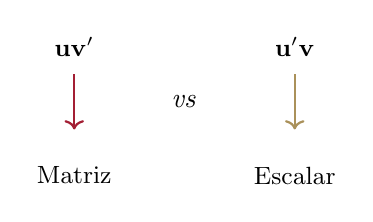
\begin{tikzpicture}[scale=0.7]
    % Producto exterior
    \node at (0,2) {\small $\mathbf{uv}'$};
    \draw[->, thick, MITCrimson] (0,1.5) -- (0,0.5);
    \node[below, font=\small] at (0,0) {Matriz};
    
    % vs
    \node at (2,1) {\textit{vs}};
    
    % Producto interior
    \node at (4,2) {\small $\mathbf{u}'\mathbf{v}$};
    \draw[->, thick, GoldLeaf] (4,1.5) -- (4,0.5);
    \node[below, font=\small] at (4,0) {Escalar};
\end{tikzpicture}
\end{center}

\section{VIII. Matrices Cuadradas}

\noindent\textbf{DEFINICIÓN.} Una matriz es cuadrada cuando tiene el mismo número de filas que de columnas ($m = n$).

\subsection{Propiedades Especiales}

\begin{itemize}
    \item Solo las matrices cuadradas pueden tener inversa
    \item El determinante solo está definido para matrices cuadradas
    \item Las potencias de matrices ($\mathbf{A}^2, \mathbf{A}^3, \ldots$) solo están definidas para matrices cuadradas
\end{itemize}

\subsection{Diagonal Principal}

\begin{definitionbox}\textbf{Diagonal Principal}
\small Los elementos $a_{ii}$ donde $i = j$ forman la diagonal principal:
\begin{equation}
\text{diag}(\mathbf{A}) = \{a_{11}, a_{22}, \ldots, a_{nn}\}
\end{equation}
\end{definitionbox}

\noindent\textbf{Visualización:}

\begin{center}
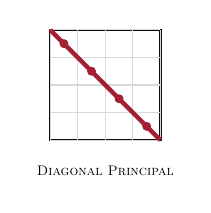
\begin{tikzpicture}[scale=0.7]
    \draw[VogueBlack, thick] (0,0) rectangle (2,2);
    \draw[step=0.5, SlateGrey!20] (0,0) grid (2,2);
    \draw[MITCrimson, ultra thick] (0,2) -- (2,0);
    \filldraw[MITCrimson] (0.25,1.75) circle (2pt);
    \filldraw[MITCrimson] (0.75,1.25) circle (2pt);
    \filldraw[MITCrimson] (1.25,0.75) circle (2pt);
    \filldraw[MITCrimson] (1.75,0.25) circle (2pt);
    \node[below, font=\tiny\scshape] at (1,-0.3) {Diagonal Principal};
\end{tikzpicture}
\end{center}

\section{IX. Matrices Diagonal y Escalar}

\noindent\textbf{MATRIZ DIAGONAL.} Una matriz cuadrada donde todos los elementos fuera de la diagonal principal son cero:

\begin{equation}
\mathbf{D} = \begin{bmatrix}
d_1 & 0 & \cdots & 0 \\
0 & d_2 & \cdots & 0 \\
\vdots & \vdots & \ddots & \vdots \\
0 & 0 & \cdots & d_n
\end{bmatrix}
\end{equation}

\noindent\textbf{MATRIZ ESCALAR.} Un caso especial de matriz diagonal donde todos los elementos diagonales son iguales:

\begin{equation}
k\mathbf{I} = \begin{bmatrix}
k & 0 & \cdots & 0 \\
0 & k & \cdots & 0 \\
\vdots & \vdots & \ddots & \vdots \\
0 & 0 & \cdots & k
\end{bmatrix}
\end{equation}

\subsection{Propiedades de Matrices Diagonales}

\begin{voguebox}\textbf{Facilidad Computacional}
\small
\begin{enumerate}
    \item La suma y producto de matrices diagonales es diagonal
    \item La inversa de una matriz diagonal (si existe) es diagonal
    \item $(\mathbf{D}^k)_{ii} = d_i^k$ para potencias enteras
\end{enumerate}
\end{voguebox}

\noindent\textbf{Inversa de Matriz Diagonal:}
\begin{equation}
\mathbf{D}^{-1} = \begin{bmatrix}
\frac{1}{d_1} & 0 & \cdots & 0 \\
0 & \frac{1}{d_2} & \cdots & 0 \\
\vdots & \vdots & \ddots & \vdots \\
0 & 0 & \cdots & \frac{1}{d_n}
\end{bmatrix}
\quad \text{si } d_i \neq 0
\end{equation}



\section{X. Matriz Triangular}

\noindent\textbf{DEFINICIÓN.} Una matriz triangular superior tiene ceros debajo de la diagonal principal:

\begin{equation}
\mathbf{U} = \begin{bmatrix}
u_{11} & u_{12} & \cdots & u_{1n} \\
0 & u_{22} & \cdots & u_{2n} \\
\vdots & \vdots & \ddots & \vdots \\
0 & 0 & \cdots & u_{nn}
\end{bmatrix}
\end{equation}

\noindent\textbf{Matriz Triangular Inferior} tiene ceros arriba de la diagonal principal:

\begin{equation}
\mathbf{L} = \begin{bmatrix}
\ell_{11} & 0 & \cdots & 0 \\
\ell_{21} & \ell_{22} & \cdots & 0 \\
\vdots & \vdots & \ddots & \vdots \\
\ell_{n1} & \ell_{n2} & \cdots & \ell_{nn}
\end{bmatrix}
\end{equation}

\subsection{Aplicación: Factorización LU}

\begin{theorembox}\textbf{Descomposición Triangular}
\small Cualquier matriz no singular puede factorizarse como producto de una matriz triangular inferior y una superior:
\begin{equation}
\mathbf{A} = \mathbf{LU}
\end{equation}
\end{theorembox}

\noindent\textbf{Visualización de la Estructura:}

\begin{center}
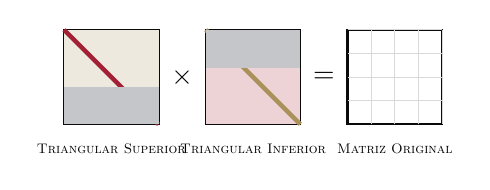
\begin{tikzpicture}[scale=0.6]
    % Triangular Superior
    \draw[VogueBlack, thick] (0,1.5) rectangle (2,3.5);
    \fill[GoldLeaf!20] (0,1.5) rectangle (2,3.5);
    \draw[MITCrimson, ultra thick] (0,3.5) -- (2,1.5);
    \fill[SlateGrey!30] (0,2.3) -- (2,2.3) -- (2,1.5) -- (0,1.5) -- cycle;
    \node[below, font=\tiny\scshape] at (1,1.3) {Triangular Superior};
    
    % Multiplicación
    \node at (2.5, 2.5) {$\times$};
    
    % Triangular Inferior
    \draw[VogueBlack, thick] (3,1.5) rectangle (5,3.5);
    \fill[MITCrimson!20] (3,1.5) rectangle (5,3.5);
    \draw[GoldLeaf, ultra thick] (3,3.5) -- (5,1.5);
    \fill[SlateGrey!30] (3,3.5) -- (5,3.5) -- (5,2.7) -- (3,2.7) -- cycle;
    \node[below, font=\tiny\scshape] at (4,1.3) {Triangular Inferior};
    
    % Igual
    \node at (5.5, 2.5) {$=$};
    
    % Matriz Original
    \draw[VogueBlack, thick] (6,1.5) rectangle (8,3.5);
    \draw[step=0.5, SlateGrey!20] (6,1.5) grid (8,3.5);
    \node[below, font=\tiny\scshape] at (7,1.3) {Matriz Original};
\end{tikzpicture}
\end{center}

\section{XI. Matrices Simétricas y Antisimétricas}

\noindent\textbf{MATRIZ SIMÉTRICA.} Una matriz cuadrada es simétrica si $\mathbf{A} = \mathbf{A}^T$:

\begin{equation}
a_{ij} = a_{ji} \quad \forall i,j
\end{equation}

\noindent\textbf{MATRIZ ANTISIMÉTRICA.} Una matriz cuadrada es antisimétrica si $\mathbf{A} = -\mathbf{A}^T$:

\begin{equation}
a_{ij} = -a_{ji} \quad \text{y} \quad a_{ii} = 0
\end{equation}

\subsection{Descomposición Única}

\begin{theorembox}\textbf{Teorema de Descomposición}
\small Toda matriz cuadrada puede expresarse como suma de una matriz simétrica y una antisimétrica:
\begin{equation}
\mathbf{A} = \frac{1}{2}(\mathbf{A} + \mathbf{A}^T) + \frac{1}{2}(\mathbf{A} - \mathbf{A}^T)
\end{equation}
\end{theorembox}



\section{XII. Ejemplos y Aplicaciones}

\noindent\textbf{EJEMPLO DE MATRIZ DIAGONAL:}

\begin{equation}
\mathbf{D} = \begin{bmatrix}
3 & 0 & 0 \\
0 & -1 & 0 \\
0 & 0 & 5
\end{bmatrix}
\end{equation}

\noindent\textbf{Potencias:}
\begin{equation}
\mathbf{D}^3 = \begin{bmatrix}
27 & 0 & 0 \\
0 & -1 & 0 \\
0 & 0 & 125
\end{bmatrix}
\end{equation}

\noindent\textbf{EJEMPLO DE MATRIZ SIMÉTRICA:}

\begin{equation}
\mathbf{S} = \begin{bmatrix}
2 & 4 & 1 \\
4 & 3 & -2 \\
1 & -2 & 5
\end{bmatrix}
\end{equation}

Note que $s_{12} = s_{21} = 4$, $s_{13} = s_{31} = 1$, $s_{23} = s_{32} = -2$.

\noindent\textbf{EJEMPLO DE MATRIZ ANTISIMÉTRICA:}

\begin{equation}
\mathbf{T} = \begin{bmatrix}
0 & 3 & -2 \\
-3 & 0 & 1 \\
2 & -1 & 0
\end{bmatrix}
\end{equation}

Note que $t_{12} = -t_{21} = 3$, y todos los elementos diagonales son cero.

\subsection{Aplicación Económica: Matriz de Varianza-Covarianza}

\begin{voguebox}\textbf{Portafolios de Inversión}
\small En finanzas, la matriz de varianza-covarianza $\mathbf{\Sigma}$ de un conjunto de activos es simétrica. El elemento $\sigma_{ij}$ representa la covarianza entre los activos $i$ y $j$, con $\sigma_{ij} = \sigma_{ji}$.

La varianza del portafolio con pesos $\mathbf{w}$ es:
\begin{equation}
\text{Var}(\text{Portafolio}) = \mathbf{w}^T\mathbf{\Sigma}\mathbf{w}
\end{equation}
\end{voguebox}

\noindent\textbf{EJEMPLO NUMÉRICO:}

\begin{equation}
\mathbf{\Sigma} = \begin{bmatrix}
0.04 & 0.015 & 0.01 \\
0.015 & 0.09 & 0.02 \\
0.01 & 0.02 & 0.16
\end{bmatrix}
\end{equation}

\noindent\textbf{Propiedades:}
\begin{itemize}
    \item Simétrica: $\sigma_{12} = \sigma_{21} = 0.015$
    \item Diagonal: varianzas individuales ($0.04, 0.09, 0.16$)
    \item Fuera de diagonal: covarianzas entre activos
\end{itemize}

\section{XIII. Representación Matricial de Sistemas}

\noindent\textbf{FORMA GENERAL.} Un sistema de $m$ ecuaciones lineales con $n$ incógnitas:

\begin{equation}
\begin{aligned}
a_{11}x_1 + a_{12}x_2 + \cdots + a_{1n}x_n &= d_1 \\
a_{21}x_1 + a_{22}x_2 + \cdots + a_{2n}x_n &= d_2 \\
&\vdots \\
a_{m1}x_1 + a_{m2}x_2 + \cdots + a_{mn}x_n &= d_m
\end{aligned}
\end{equation}

\noindent\textbf{Forma Matricial Compacta:}

\begin{equation}
\mathbf{Ax} = \mathbf{d}
\end{equation}

donde:
\begin{itemize}
    \item $\mathbf{A}_{m \times n}$: matriz de coeficientes
    \item $\mathbf{x}_{n \times 1}$: vector de incógnitas
    \item $\mathbf{d}_{m \times 1}$: vector de términos constantes
\end{itemize}

\subsection{Interpretación Geométrica}

\begin{voguebox}\textbf{Interpretación en $\mathbb{R}^n$}
\small Cada ecuación representa un hiperplano en $\mathbb{R}^n$. La solución del sistema corresponde a la intersección de todos estos hiperplanos.
\end{voguebox}

\noindent\textbf{CASOS EN $\mathbb{R}^2$:}
\begin{itemize}
    \item \textbf{Solución única:} Dos rectas que se intersecan en un punto
    \item \textbf{Infinitas soluciones:} Dos rectas coincidentes
    \item \textbf{Sin solución:} Dos rectas paralelas
\end{itemize}

\section{XIV. Tipos de Sistemas}

\noindent\textbf{CLASIFICACIÓN POR NÚMERO DE ECUACIONES:}

\begin{definitionbox}\textbf{Sistemas Cuadrados}
\small Cuando $m = n$ (mismo número de ecuaciones que de incógnitas). Este es el caso más común en modelos económicos de equilibrio.
\end{definitionbox}

\begin{definitionbox}\textbf{Sistemas Sobredeterminados}
\small Cuando $m > n$ (más ecuaciones que incógnitas). Puede no tener solución o tener solución exacta si hay dependencias lineales.
\end{definitionbox}

\begin{definitionbox}\textbf{Sistemas Subdeterminados}
\small Cuando $m < n$ (menos ecuaciones que incógnitas). Generalmente tiene infinitas soluciones.
\end{definitionbox}

\subsection{Visualización de Casos}

\begin{center}
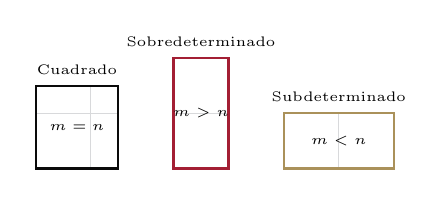
\begin{tikzpicture}[scale=0.7]
    % Sistema Cuadrado
    \begin{scope}
        \draw[SlateGrey!20] (0,0) grid (1.5,1.5);
        \draw[VogueBlack, thick] (0,0) rectangle (1.5,1.5);
        \node[font=\tiny] at (0.75,1.8) {Cuadrado};
        \node[font=\tiny] at (0.75,0.75) {$m = n$};
    \end{scope}
    
    % Sistema Sobredeterminado
    \begin{scope}[xshift=2.5cm]
        \draw[SlateGrey!20] (0,0) grid (1,2);
        \draw[MITCrimson, thick] (0,0) rectangle (1,2);
        \node[font=\tiny] at (0.5,2.3) {Sobredeterminado};
        \node[font=\tiny] at (0.5,1) {$m > n$};
    \end{scope}
    
    % Sistema Subdeterminado
    \begin{scope}[xshift=4.5cm]
        \draw[SlateGrey!20] (0,0) grid (2,1);
        \draw[GoldLeaf, thick] (0,0) rectangle (2,1);
        \node[font=\tiny] at (1,1.3) {Subdeterminado};
        \node[font=\tiny] at (1,0.5) {$m < n$};
    \end{scope}
\end{tikzpicture}
\end{center}



\section{XV. Métodos de Solución}

\noindent\textbf{1. MÉTODO DE SUSTITUCIÓN}

El método tradicional para sistemas pequeños. Se despeja una variable y se sustituye en las demás ecuaciones.

\noindent\textbf{EJEMPLO: Sistema 2×2}
\begin{equation}
\begin{aligned}
2x + y &= 8 \\
x - y &= 1
\end{aligned}
\end{equation}

Solución: De la segunda: $x = y + 1$. Sustituyendo:
\begin{align*}
2(y + 1) + y &= 8 \\
2y + 2 + y &= 8 \\
3y &= 6 \\
y &= 2, \quad x = 3
\end{align*}

\noindent\textbf{2. MÉTODO DE ELIMINACIÓN GAUSSIANA}

Transformación del sistema a forma escalonada mediante operaciones elementales de fila.

\begin{theorembox}\textbf{Operaciones Elementales}
\small
\begin{enumerate}
    \item Intercambiar dos ecuaciones (filas)
    \item Multiplicar una ecuación por escalar no nulo
    \item Sumar un múltiplo de una ecuación a otra
\end{enumerate}
\end{theorembox}

\noindent\textbf{EJEMPLO:}

\begin{equation}
\begin{bmatrix}
1 & 2 & 3 \\
2 & 5 & 8 \\
1 & 1 & 2
\end{bmatrix}
\begin{bmatrix}
x \\ y \\ z
\end{bmatrix}
=
\begin{bmatrix}
6 \\ 15 \\ 4
\end{bmatrix}
\end{equation}

\noindent\textbf{3. MÉTODO DE LA INVERSA (para sistemas cuadrados)}

Si $\mathbf{A}$ es no singular ($\det(\mathbf{A}) \neq 0$):

\begin{equation}
\mathbf{x} = \mathbf{A}^{-1}\mathbf{d}
\end{equation}

\section{XVI. Sistemas Homogéneos}

\noindent\textbf{DEFINICIÓN.} Un sistema es homogéneo si $\mathbf{d} = \mathbf{0}$:

\begin{equation}
\mathbf{Ax} = \mathbf{0}
\end{equation}

\noindent\textbf{PROPIEDADES:}

\begin{voguebox}\textbf{Teorema Fundamental}
\small
\begin{enumerate}
    \item Todo sistema homogéneo tiene al menos la solución trivial $\mathbf{x} = \mathbf{0}$
    \item Si $\mathbf{A}$ es no singular, solo tiene la solución trivial
    \item Si $\mathbf{A}$ es singular, tiene infinitas soluciones no triviales
\end{enumerate}
\end{voguebox}

\noindent\textbf{EJEMPLO: Sistema Homogéneo 2×2}
\begin{equation}
\begin{bmatrix}
2 & 1 \\
4 & 2
\end{bmatrix}
\begin{bmatrix}
x \\ y
\end{bmatrix}
=
\begin{bmatrix}
0 \\ 0
\end{bmatrix}
\end{equation}

La segunda ecuación es múltiplo de la primera: $4x + 2y = 2(2x + y)$. El sistema es singular y tiene infinitas soluciones: $y = -2x$.



\section{XVII. Aplicaciones Económicas}

\noindent\textbf{1. MODELO DE MERCADO DE $n$ BIENES}

Para $n$ bienes interdependientes:

\begin{equation}
\begin{aligned}
Q_{d1} &= a_1 + b_{11}P_1 + b_{12}P_2 + \cdots + b_{1n}P_n \\
Q_{d2} &= a_2 + b_{21}P_1 + b_{22}P_2 + \cdots + b_{2n}P_n \\
&\vdots \\
Q_{dn} &= a_n + b_{n1}P_1 + b_{n2}P_2 + \cdots + b_{nn}P_n
\end{aligned}
\end{equation}

\begin{equation}
Q_{si} = c_i + d_{i1}P_1 + d_{i2}P_2 + \cdots + d_{in}P_n \quad (i = 1,\ldots,n)
\end{equation}

Condición de equilibrio: $Q_{di} = Q_{si}$ para todo $i$.


\begin{equation}
\mathbf{Q}_d = \mathbf{a} + \mathbf{BP}, \quad \mathbf{Q}_s = \mathbf{c} + \mathbf{DP}
\end{equation}

\begin{equation}
\mathbf{a} + \mathbf{BP} = \mathbf{c} + \mathbf{DP} \quad \Rightarrow \quad (\mathbf{B} - \mathbf{D})\mathbf{P} = \mathbf{c} - \mathbf{a}
\end{equation}

\noindent\textbf{2. MODELO DE INSUMO-PRODUCTO (Leontief)}

Para una economía con $n$ sectores:

\begin{equation}
\mathbf{x} = \mathbf{Ax} + \mathbf{d}
\end{equation}

donde:
\begin{itemize}
    \item $\mathbf{x}$: vector de producción total
    \item $\mathbf{A}$: matriz de coeficientes técnicos
    \item $\mathbf{d}$: vector de demanda final
\end{itemize}

Solución:
\begin{equation}
\mathbf{x} = (\mathbf{I} - \mathbf{A})^{-1}\mathbf{d}
\end{equation}

\subsection{Condición de Existencia}

\begin{theorembox}\textbf{Teorema de Hawkins-Simon}
\small Para que exista solución no negativa en el modelo de Leontief, es necesario y suficiente que:
\begin{enumerate}
    \item $\det(\mathbf{I} - \mathbf{A}) > 0$
    \item Todos los menores principales de $(\mathbf{I} - \mathbf{A})$ sean positivos
\end{enumerate}
\end{theorembox}

\noindent\textbf{EJEMPLO: Economía de 2 Sectores}

\begin{equation}
\begin{bmatrix}
x_1 \\ x_2
\end{bmatrix}
=
\begin{bmatrix}
0.3 & 0.2 \\
0.1 & 0.4
\end{bmatrix}
\begin{bmatrix}
x_1 \\ x_2
\end{bmatrix}
+
\begin{bmatrix}
100 \\ 50
\end{bmatrix}
\end{equation}

Solución:
\begin{equation}
\begin{split}
\begin{bmatrix}
x_1 \\ x_2
\end{bmatrix}
&=
\left(
\begin{bmatrix}
1 & 0 \\
0 & 1
\end{bmatrix}
-
\begin{bmatrix}
0.3 & 0.2 \\
0.1 & 0.4
\end{bmatrix}
\right)^{-1}
\begin{bmatrix}
100 \\ 50
\end{bmatrix} \\ % <-- Salto de línea
&= \begin{bmatrix}
0.7 & -0.2 \\
-0.1 & 0.6
\end{bmatrix}^{-1}
\begin{bmatrix}
100 \\ 50
\end{bmatrix}
\end{split}
\end{equation}


\section{XVIII. Definición y Propiedades}

\noindent\textbf{DEFINICIÓN.} El determinante es una función escalar que asigna a cada matriz cuadrada $\mathbf{A}$ un número real, denotado $|\mathbf{A}|$ o $\det(\mathbf{A})$.

\subsection{Determinante 2×2}

\begin{equation}
|\mathbf{A}| = \begin{vmatrix}
a_{11} & a_{12} \\
a_{21} & a_{22}
\end{vmatrix}
= a_{11}a_{22} - a_{12}a_{21}
\end{equation}

\noindent\textbf{EJEMPLO:}
\begin{equation}
\begin{vmatrix}
3 & 1 \\
2 & 4
\end{vmatrix}
= 3 \cdot 4 - 1 \cdot 2 = 12 - 2 = 10
\end{equation}

\subsection{Determinante 3×3 (Regla de Sarrus)}

\begin{multline}
\begin{vmatrix}
a_{11} & a_{12} & a_{13} \\
a_{21} & a_{22} & a_{23} \\
a_{31} & a_{32} & a_{33}
\end{vmatrix}
= a_{11}a_{22}a_{33} + a_{12}a_{23}a_{31} + a_{13}a_{21}a_{32} \\
- a_{31}a_{22}a_{13} - a_{32}a_{23}a_{11} - a_{33}a_{21}a_{12}
\end{multline}



\noindent\textbf{Visualización Gráfica:}

\begin{center}
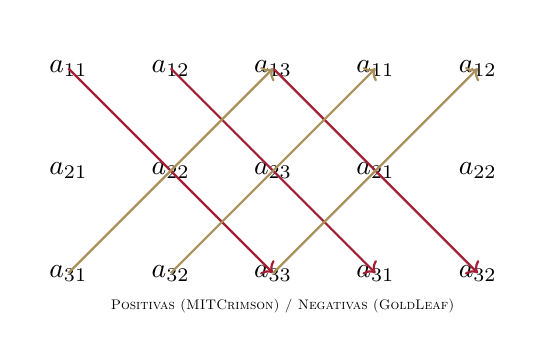
\begin{tikzpicture}[scale=0.6]
    \matrix [matrix of math nodes, nodes in empty cells,
             column sep=0.5cm, row sep=0.5cm,
             nodes={minimum size=0.8cm}] (m) {
        a_{11} & a_{12} & a_{13} & a_{11} & a_{12} \\
        a_{21} & a_{22} & a_{23} & a_{21} & a_{22} \\
        a_{31} & a_{32} & a_{33} & a_{31} & a_{32} \\
    };
    
    % Diagonales positivas
    \draw[MITCrimson, thick, ->] (m-1-1.center) -- (m-2-2.center) -- (m-3-3.center);
    \draw[MITCrimson, thick, ->] (m-1-2.center) -- (m-2-3.center) -- (m-3-4.center);
    \draw[MITCrimson, thick, ->] (m-1-3.center) -- (m-2-4.center) -- (m-3-5.center);
    
    % Diagonales negativas
    \draw[GoldLeaf, thick, ->] (m-3-1.center) -- (m-2-2.center) -- (m-1-3.center);
    \draw[GoldLeaf, thick, ->] (m-3-2.center) -- (m-2-3.center) -- (m-1-4.center);
    \draw[GoldLeaf, thick, ->] (m-3-3.center) -- (m-2-4.center) -- (m-1-5.center);
    
    \node[below, font=\tiny\scshape] at (0.2,-2.5) {Positivas (MITCrimson) / Negativas (GoldLeaf)};
\end{tikzpicture}
\end{center}

\subsection{Propiedades Fundamentales}

\begin{voguebox}\textbf{Propiedades del Determinante}

\small
\begin{enumerate}
    \item $|\mathbf{I}| = 1$
    \item $|\mathbf{A}^T| = |\mathbf{A}|$
    \item Si dos filas (o columnas) son iguales, $|\mathbf{A}| = 0$
    \item Si una fila es múltiplo de otra, $|\mathbf{A}| = 0$
    \item $|\mathbf{AB}| = |\mathbf{A}||\mathbf{B}|$
    \item $|\mathbf{A}^{-1}| = \frac{1}{|\mathbf{A}|}$ si $\mathbf{A}$ es no singular
\end{enumerate}
\end{voguebox}



\secbar



% --- PIE DE PÁGINA ---

\end{multicols*}

\begin{tikzpicture}[remember picture, overlay]
    \fill[VogueBlack] ($(current page.north west)$) rectangle ($(current page.north east) + (0,-0.3in)$);
    \node[white, anchor=west] at ($(current page.north west) + (0.5in, -0.15in)$) {\fontfamily{phv}\selectfont \textbf{DIVISIÓN DE ECONOMÍA MATEMÁTICA COMPUTACIONAL}};
    \node[white, anchor=east] at ($(current page.north east) + (-0.5in, -0.15in)$) {\textsc{\small Sección 4.4: Valores y Vectores Propios}};
\end{tikzpicture}

\begin{multicols*}{3}

\section{XIX. Expansión por Cofactores}

\noindent\textbf{DEFINICIÓN.} Para una matriz $n \times n$:

\begin{equation}
|\mathbf{A}| = \sum_{j=1}^{n} a_{ij}C_{ij} \quad \text{(expansión por la fila $i$)}
\end{equation}

\begin{equation}
|\mathbf{A}| = \sum_{i=1}^{n} a_{ij}C_{ij} \quad \text{(expansión por la columna $j$)}
\end{equation}

donde $C_{ij} = (-1)^{i+j}M_{ij}$ es el cofactor.

\subsection{Menor y Cofactor}

\begin{definitionbox}\textbf{Menor $M_{ij}$}
\small El menor $M_{ij}$ es el determinante de la submatriz obtenida al eliminar la fila $i$ y columna $j$ de $\mathbf{A}$.
\end{definitionbox}

\begin{definitionbox}\textbf{Cofactor $C_{ij}$}
\small El cofactor es el menor con signo: $C_{ij} = (-1)^{i+j}M_{ij}$.
\end{definitionbox}

\noindent\textbf{EJEMPLO: Matriz 3×3}

\begin{equation}
\mathbf{A} = \begin{bmatrix}
1 & 2 & 3 \\
4 & 5 & 6 \\
7 & 8 & 9
\end{bmatrix}
\end{equation}

\noindent\textbf{Cálculo de $C_{11}$:}
\begin{align*}
M_{11} &= \begin{vmatrix} 5 & 6 \\ 8 & 9 \end{vmatrix} = 5\cdot9 - 6\cdot8 = 45 - 48 = -3 \\
C_{11} &= (-1)^{1+1}(-3) = -3
\end{align*}

\noindent\textbf{Cálculo de $C_{23}$:}
\begin{align*}
M_{23} &= \begin{vmatrix} 1 & 2 \\ 7 & 8 \end{vmatrix} = 1\cdot8 - 2\cdot7 = 8 - 14 = -6 \\
C_{23} &= (-1)^{2+3}(-6) = (-1)^5(-6) = 6
\end{align*}

\section{XX. Matriz Adjunta y Regla de Cramer}

\noindent\textbf{MATRIZ ADJUNTA.} La matriz adjunta de $\mathbf{A}$ es la transpuesta de la matriz de cofactores:



\begin{equation}
\text{adj}(\mathbf{A}) = [C_{ji}] \quad \text{(¡cuidado con los índices!)}
\end{equation}

\noindent\textbf{FÓRMULA DE LA INVERSA:}

\begin{equation}
\mathbf{A}^{-1} = \frac{1}{|\mathbf{A}|}\text{adj}(\mathbf{A}) \quad \text{si } |\mathbf{A}| \neq 0
\end{equation}

\noindent\textbf{REGLA DE CRAMER.} Para resolver $\mathbf{Ax} = \mathbf{d}$:

\begin{equation}
x_j = \frac{|\mathbf{A}_j|}{|\mathbf{A}|} \quad (j = 1,\ldots,n)
\end{equation}

donde $\mathbf{A}_j$ es la matriz obtenida al reemplazar la columna $j$ de $\mathbf{A}$ por $\mathbf{d}$.



\noindent\textbf{EJEMPLO DE REGLA DE CRAMER:}

Sistema:
\begin{equation}
\begin{bmatrix}
2 & 1 \\
1 & -1
\end{bmatrix}
\begin{bmatrix}
x \\ y
\end{bmatrix}
=
\begin{bmatrix}
4 \\ 1
\end{bmatrix}
\end{equation}

\noindent\textbf{Cálculos:}
\begin{align*}
|\mathbf{A}| &= \begin{vmatrix} 2 & 1 \\ 1 & -1 \end{vmatrix} = 2(-1) - 1(1) = -2 - 1 = -3 \\
|\mathbf{A}_1| &= \begin{vmatrix} 4 & 1 \\ 1 & -1 \end{vmatrix} = 4(-1) - 1(1) = -4 - 1 = -5 \\
|\mathbf{A}_2| &= \begin{vmatrix} 2 & 4 \\ 1 & 1 \end{vmatrix} = 2(1) - 4(1) = 2 - 4 = -2
\end{align*}

\noindent\textbf{Solución:}
\begin{align*}
x &= \frac{|\mathbf{A}_1|}{|\mathbf{A}|} = \frac{-5}{-3} = \frac{5}{3} \\
y &= \frac{|\mathbf{A}_2|}{|\mathbf{A}|} = \frac{-2}{-3} = \frac{2}{3}
\end{align*}

\section{XXI. Interpretación Geométrica}
\noindent\textbf{EN $\mathbb{R}^2$:} El valor absoluto del determinante 2×2 representa el área del paralelogramo formado por los vectores columna.

\noindent\textbf{Visualización:}

\begin{center}
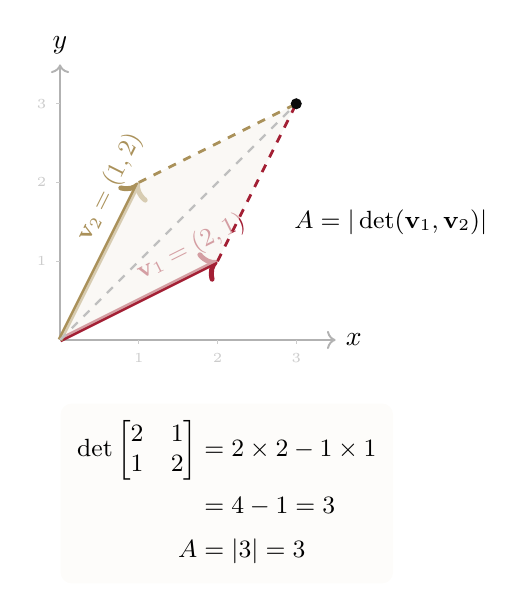
\begin{tikzpicture}[scale=1.0]  % Aumenté la escala para mejor visibilidad
    % Ejes con etiquetas más claras
    \draw[->, gray!60, line width=0.7pt] (0,0) -- (3.5,0) node[right, black] {$x$};
    \draw[->, gray!60, line width=0.7pt] (0,0) -- (0,3.5) node[above, black] {$y$};
    
    % Marcas en los ejes
    \foreach \x in {1,2,3}
        \draw[gray!40] (\x,0) -- (\x,-0.05) node[below, font=\tiny] {$\x$};
    \foreach \y in {1,2,3}
        \draw[gray!40] (0,\y) -- (-0.05,\y) node[left, font=\tiny] {$\y$};
    
    % Vectores más destacados
    \draw[->, MITCrimson, line width=1.8pt] (0,0) -- (2,1) 
        node[midway, above right, sloped, font=\small] {$\mathbf{v}_1 = (2,1)$};
    \draw[->, GoldLeaf, line width=1.8pt] (0,0) -- (1,2) 
        node[midway, above right, sloped, font=\small] {$\mathbf{v}_2 = (1,2)$};
    
    % Paralelogramo con relleno sutil
    \fill[GoldLeaf!10, opacity=0.6] (0,0) -- (2,1) -- (3,3) -- (1,2) -- cycle;
    
    % Líneas del paralelogramo
    \draw[dashed, MITCrimson, line width=1pt] (2,1) -- (3,3);
    \draw[dashed, GoldLeaf, line width=1pt] (1,2) -- (3,3);
    \draw[dashed, gray!50, line width=0.8pt] (0,0) -- (3,3);
    
    % Punto final del paralelogramo
    \fill[VogueBlack] (3,3) circle (2pt);
    
    % Etiqueta del área con fondo más legible
    \node[fill=white, fill opacity=0.9, text opacity=1, 
          inner sep=5pt, rounded corners=3pt, font=\small] 
          at (4.2,1.5) {$A = |\det(\mathbf{v}_1,\mathbf{v}_2)|$};
    
    % Cálculo del determinante en una caja
    \node[fill=SoftLinen, inner sep=6pt, rounded corners=4pt, 
          anchor=north west, font=\small] at (0,-0.8) {
        $\begin{aligned}
            \det\begin{bmatrix}2 & 1\\1 & 2\end{bmatrix} &= 2\times2 - 1\times1 \\
            &= 4 - 1 = 3 \\[2pt]
            A &= |3| = 3
        \end{aligned}$
    };
\end{tikzpicture}
\end{center}

\noindent\textbf{EN $\mathbb{R}^3$:} El valor absoluto del determinante 3×3 representa el volumen del paralelepípedo formado por los tres vectores columna.

\subsection{Interpretación en Transformaciones Lineales}

\begin{voguebox}\textbf{Factor de Expansión/Contracción}
\small Si $T: \mathbb{R}^n \to \mathbb{R}^n$ es una transformación lineal con matriz $\mathbf{A}$, entonces $|\det(\mathbf{A})|$ representa el factor por el cual se escala el volumen (área en $\mathbb{R}^2$) bajo $T$.
\end{voguebox}


% aqui termina

\section{XXII. Definición Fundamental}

\noindent\textbf{PROBLEMA DE VALOR PROPIO.} Dada una matriz cuadrada $\mathbf{A}_{n \times n}$, encontrar escalares $\lambda$ (valores propios) y vectores no nulos $\mathbf{v}$ (vectores propios) tales que:

\begin{equation}
\mathbf{Av} = \lambda\mathbf{v}
\end{equation}

\noindent\textbf{Interpretación:} $\mathbf{v}$ es un vector que bajo la transformación $\mathbf{A}$ solo se escala (no cambia dirección).

\subsection{Formulación Alternativa}

\begin{equation}
(\mathbf{A} - \lambda\mathbf{I})\mathbf{v} = \mathbf{0}
\end{equation}

Esta es un sistema homogéneo. Para tener soluciones no triviales ($\mathbf{v} \neq \mathbf{0}$):

\begin{equation}
|\mathbf{A} - \lambda\mathbf{I}| = 0
\end{equation}

\noindent\textbf{ECUACIÓN CARACTERÍSTICA:}

\begin{equation}
P(\lambda) = \det(\mathbf{A} - \lambda\mathbf{I}) = 0
\end{equation}

\section{XXIII. Cálculo de Valores Propios}

\noindent\textbf{PASO 1:} Formar $\mathbf{A} - \lambda\mathbf{I}$

\noindent\textbf{PASO 2:} Calcular el determinante

\noindent\textbf{PASO 3:} Resolver la ecuación polinomial $P(\lambda) = 0$

\noindent\textbf{EJEMPLO: Matriz 2×2}

\begin{equation}
\mathbf{A} = \begin{bmatrix}
4 & 1 \\
2 & 3
\end{bmatrix}
\end{equation}

\begin{align*}
\mathbf{A} - \lambda\mathbf{I} &= \begin{bmatrix}
4 - \lambda & 1 \\
2 & 3 - \lambda
\end{bmatrix} \\
|\mathbf{A} - \lambda\mathbf{I}| &= (4 - \lambda)(3 - \lambda) - 2\cdot1 \\
&= \lambda^2 - 7\lambda + 10 \\
&= (\lambda - 2)(\lambda - 5) = 0
\end{align*}

\noindent\textbf{Valores propios:} $\lambda_1 = 2$, $\lambda_2 = 5$

\subsection{Ejemplo 3×3}

\begin{equation}
\mathbf{B} = \begin{bmatrix}
2 & 0 & 0 \\
0 & 3 & 4 \\
0 & 4 & 9
\end{bmatrix}
\end{equation}

\begin{align*}
|\mathbf{B} - \lambda\mathbf{I}| &= 
\begin{vmatrix}
2 - \lambda & 0 & 0 \\
0 & 3 - \lambda & 4 \\
0 & 4 & 9 - \lambda
\end{vmatrix} \\
&= (2 - \lambda)\begin{vmatrix}
3 - \lambda & 4 \\
4 & 9 - \lambda
\end{vmatrix} \\
&= (2 - \lambda)[(3 - \lambda)(9 - \lambda) - 16] \\
&= (2 - \lambda)(\lambda^2 - 12\lambda + 11) \\
&= (2 - \lambda)(\lambda - 1)(\lambda - 11) = 0
\end{align*}

\noindent\textbf{Valores propios:} $\lambda_1 = 1$, $\lambda_2 = 2$, $\lambda_3 = 11$



\section{XXIV. Cálculo de Vectores Propios}

\noindent\textbf{PARA CADA VALOR PROPIO $\lambda_i$:}

Resolver el sistema homogéneo $(\mathbf{A} - \lambda_i\mathbf{I})\mathbf{v} = \mathbf{0}$

\noindent\textbf{EJEMPLO (continuación):} Para $\lambda_1 = 2$ en el ejemplo anterior:

\begin{equation}
(\mathbf{A} - 2\mathbf{I})\mathbf{v} = \begin{bmatrix}
2 & 1 \\
2 & 1
\end{bmatrix}
\begin{bmatrix}
v_1 \\ v_2
\end{bmatrix}
=
\begin{bmatrix}
0 \\ 0
\end{bmatrix}
\end{equation}

Esto da: $2v_1 + v_2 = 0 \Rightarrow v_2 = -2v_1$

Elegimos $v_1 = 1$, entonces $v_2 = -2$:

\begin{equation}
\mathbf{v}_1 = \begin{bmatrix}
1 \\ -2
\end{bmatrix}
\end{equation}

\noindent\textbf{Para $\lambda_2 = 5$:}

\begin{equation}
(\mathbf{A} - 5\mathbf{I})\mathbf{v} = \begin{bmatrix}
-1 & 1 \\
2 & -2
\end{bmatrix}
\begin{bmatrix}
v_1 \\ v_2
\end{bmatrix}
=
\begin{bmatrix}
0 \\ 0
\end{bmatrix}
\end{equation}

Esto da: $-v_1 + v_2 = 0 \Rightarrow v_2 = v_1$

Elegimos $v_1 = 1$, entonces $v_2 = 1$:

\begin{equation}
\mathbf{v}_2 = \begin{bmatrix}
1 \\ 1
\end{bmatrix}
\end{equation}

\subsection{Visualización Geométrica}

\begin{center}
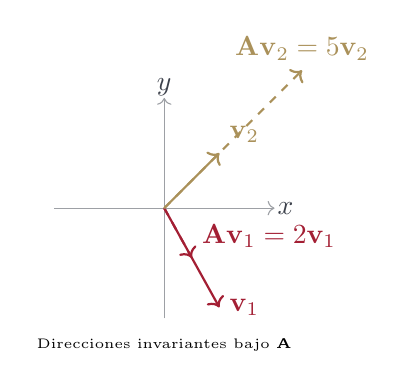
\begin{tikzpicture}[scale=0.7]
    % Ejes originales
    \draw[->, thin, SlateGrey!50] (-2,0) -- (2,0);
    \draw[->, thin, SlateGrey!50] (0,-2) -- (0,2);
    \node[SlateGrey] at (2.2,0) {$x$};
    \node[SlateGrey] at (0,2.2) {$y$};
    
    % Vector propio v1
    \draw[->, MITCrimson, thick] (0,0) -- (1,-1.8) node[right] {$\mathbf{v}_1$};
    \draw[->, MITCrimson, dashed, thick] (0,0) -- (0.5,-0.9) node[above right] {$\mathbf{Av}_1 = 2\mathbf{v}_1$};
    
    % Vector propio v2
    \draw[->, GoldLeaf, thick] (0,0) -- (1,1) node[above right] {$\mathbf{v}_2$};
    \draw[->, GoldLeaf, dashed, thick] (0,0) -- (2.5,2.5) node[above] {$\mathbf{Av}_2 = 5\mathbf{v}_2$};
    
    % Notas
    \node[below, font=\tiny] at (0,-2.2) {Direcciones invariantes bajo $\mathbf{A}$};
\end{tikzpicture}
\end{center}

\section{XXV. Propiedades Importantes}

\noindent\textbf{1. TRAZA Y DETERMINANTE:}

\begin{equation}
\text{tr}(\mathbf{A}) = \sum_{i=1}^{n} \lambda_i, \quad \det(\mathbf{A}) = \prod_{i=1}^{n} \lambda_i
\end{equation}

\noindent\textbf{2. MATRICES SIMÉTRICAS:} Los valores propios son reales y los vectores propios son ortogonales.

\noindent\textbf{3. MATRICES DIAGONALES:} Los valores propios son los elementos diagonales.

\noindent\textbf{4. POTENCIAS DE MATRICES:} Si $\mathbf{Av} = \lambda\mathbf{v}$, entonces $\mathbf{A}^k\mathbf{v} = \lambda^k\mathbf{v}$.

\noindent\textbf{5. INVERSA:} Si $\mathbf{A}$ es no singular y $\lambda \neq 0$ es valor propio de $\mathbf{A}$, entonces $\frac{1}{\lambda}$ es valor propio de $\mathbf{A}^{-1}$ con el mismo vector propio.



\section{XXVI. Diagonalización}

\noindent\textbf{TEOREMA DE DIAGONALIZACIÓN.} Si $\mathbf{A}_{n \times n}$ tiene $n$ vectores propios linealmente independientes, entonces:

\begin{equation}
\mathbf{A} = \mathbf{PDP}^{-1}
\end{equation}

donde:
\begin{itemize}
    \item $\mathbf{D}$: matriz diagonal con los valores propios
    \item $\mathbf{P}$: matriz cuyas columnas son los vectores propios
\end{itemize}

\noindent\textbf{EJEMPLO:}

Del ejemplo anterior:
\begin{align*}
\mathbf{D} &= \begin{bmatrix}
2 & 0 \\
0 & 5
\end{bmatrix}, \quad
\mathbf{P} = \begin{bmatrix}
1 & 1 \\
-2 & 1
\end{bmatrix} \\
\mathbf{P}^{-1} &= \frac{1}{3}\begin{bmatrix}
1 & -1 \\
2 & 1
\end{bmatrix}
\end{align*}

Verificación:
\begin{equation}
\mathbf{PDP}^{-1} = \begin{bmatrix}
1 & 1 \\
-2 & 1
\end{bmatrix}
\begin{bmatrix}
2 & 0 \\
0 & 5
\end{bmatrix}
\frac{1}{3}\begin{bmatrix}
1 & -1 \\
2 & 1
\end{bmatrix}
= \begin{bmatrix}
4 & 1 \\
2 & 3
\end{bmatrix}
= \mathbf{A}
\end{equation}

\subsection{Aplicación: Cálculo de Potencias}

\begin{voguebox}[title=Potencia de Matriz Diagonalizable]
\small Si $\mathbf{A} = \mathbf{PDP}^{-1}$, entonces:
\begin{equation}
\mathbf{A}^k = \mathbf{PD}^k\mathbf{P}^{-1}
\end{equation}
Y como $\mathbf{D}^k$ es fácil de calcular, esta fórmula simplifica enormemente el cálculo de $\mathbf{A}^k$.
\end{voguebox}

\noindent\textbf{EJEMPLO:}
\begin{equation}
\mathbf{A}^{10} = \mathbf{PD}^{10}\mathbf{P}^{-1} = 
\begin{bmatrix}
1 & 1 \\
-2 & 1
\end{bmatrix}
\begin{bmatrix}
2^{10} & 0 \\
0 & 5^{10}
\end{bmatrix}
\frac{1}{3}\begin{bmatrix}
1 & -1 \\
2 & 1
\end{bmatrix}
\end{equation}

\section{XXVII. Aplicaciones Económicas}

\noindent\textbf{1. MODELOS DE CRECIMIENTO}

En modelos dinámicos lineales $\mathbf{x}_{t+1} = \mathbf{Ax}_t$, el crecimiento a largo plazo está determinado por el valor propio dominante (el de mayor módulo).

\noindent\textbf{2. ANÁLISIS DE COMPONENTES PRINCIPALES}

En estadística multivariada, los valores y vectores propios de la matriz de covarianza permiten reducir la dimensionalidad de los datos.

\noindent\textbf{3. MODELOS INPUT-OUTPUT}

Los valores propios de la matriz de Leontief $\mathbf{A}$ determinan la estabilidad del sistema productivo.

\subsection{Ejemplo: Modelo de Crecimiento de Población}

\begin{equation}
\begin{bmatrix}
P_{t+1} \\ Q_{t+1}
\end{bmatrix}
=
\begin{bmatrix}
0.9 & 0.2 \\
0.1 & 0.8
\end{bmatrix}
\begin{bmatrix}
P_t \\ Q_t
\end{bmatrix}
\end{equation}

Valores propios: $\lambda_1 = 1$, $\lambda_2 = 0.7$

Interpretación: $\lambda_1 = 1$ indica un estado estacionario, $\lambda_2 = 0.7$ indica convergencia.



\section{XXVIII. Definición y Representación}

\noindent\textbf{DEFINICIÓN.} Una forma cuadrática en $n$ variables es una función homogénea de grado 2:

\begin{equation}
Q(x_1, \ldots, x_n) = \sum_{i=1}^{n} \sum_{j=1}^{n} a_{ij}x_ix_j
\end{equation}

\noindent\textbf{FORMA MATRICIAL:}

\begin{equation}
Q(\mathbf{x}) = \mathbf{x}^T\mathbf{Ax}
\end{equation}

donde $\mathbf{A}$ es una matriz simétrica (puede siempre simetrizarse sin cambiar $Q$).

\subsection{Ejemplo en 2 Variables}

\begin{equation}
Q(x, y) = ax^2 + 2bxy + cy^2 = \begin{bmatrix} x & y \end{bmatrix}
\begin{bmatrix}
a & b \\
b & c
\end{bmatrix}
\begin{bmatrix}
x \\ y
\end{bmatrix}
\end{equation}

\noindent\textbf{EJEMPLO NUMÉRICO:}
\begin{equation}
Q(x, y) = 3x^2 + 4xy + 2y^2 = \begin{bmatrix} x & y \end{bmatrix}
\begin{bmatrix}
3 & 2 \\
2 & 2
\end{bmatrix}
\begin{bmatrix}
x \\ y
\end{bmatrix}
\end{equation}

\section{XXIX. Clasificación de Formas Cuadráticas}

\noindent\textbf{DEFINICIÓN (Signo):} Para todo $\mathbf{x} \neq \mathbf{0}$:

\begin{itemize}
    \item \textbf{Definida Positiva:} $Q(\mathbf{x}) > 0$
    \item \textbf{Semidefinida Positiva:} $Q(\mathbf{x}) \geq 0$
    \item \textbf{Definida Negativa:} $Q(\mathbf{x}) < 0$
    \item \textbf{Semidefinida Negativa:} $Q(\mathbf{x}) \leq 0$
    \item \textbf{Indefinida:} $Q(\mathbf{x})$ toma valores positivos y negativos
\end{itemize}

\subsection{Criterio de los Valores Propios}

\begin{theorembox}[title=Caracterización por Valores Propios]
\small Sea $\mathbf{A}$ simétrica con valores propios $\lambda_1, \ldots, \lambda_n$:
\begin{itemize}
    \item Def. positiva $\Leftrightarrow$ $\lambda_i > 0$ $\forall i$
    \item Semidef. positiva $\Leftrightarrow$ $\lambda_i \geq 0$ $\forall i$
    \item Def. negativa $\Leftrightarrow$ $\lambda_i < 0$ $\forall i$
    \item Semidef. negativa $\Leftrightarrow$ $\lambda_i \leq 0$ $\forall i$
    \item Indefinida $\Leftrightarrow$ $\lambda_i$ de signos mezclados
\end{itemize}
\end{theorembox}

\noindent\textbf{EJEMPLO:} Para $\mathbf{A} = \begin{bmatrix}3 & 1 \\ 1 & 3\end{bmatrix}$:

Valores propios: $\lambda_1 = 2$, $\lambda_2 = 4$ (ambos positivos) $\Rightarrow$ definida positiva.



\section{XXX. Criterio de los Menores Principales}

\noindent\textbf{DEFINICIÓN.} Los menores principales de $\mathbf{A}$ son los determinantes de las submatrices obtenidas tomando las primeras $k$ filas y columnas.

\noindent\textbf{TEOREMA (Sylvester):} Para $\mathbf{A}$ simétrica:

\begin{itemize}
    \item \textbf{Definida positiva} $\Leftrightarrow$ Todos los menores principales son $> 0$
    \item \textbf{Definida negativa} $\Leftrightarrow$ Los menores principales alternan signo: $D_1 < 0$, $D_2 > 0$, $D_3 < 0$, etc.
\end{itemize}

\noindent\textbf{EJEMPLO:} Para $\mathbf{A} = \begin{bmatrix}3 & 1 \\ 1 & 3\end{bmatrix}$:

\begin{align*}
D_1 &= |3| = 3 > 0 \\
D_2 &= \begin{vmatrix}3 & 1 \\ 1 & 3\end{vmatrix} = 9 - 1 = 8 > 0
\end{align*}

$\Rightarrow$ definida positiva.

\subsection{Ejemplo 3×3}

\begin{equation}
\mathbf{A} = \begin{bmatrix}
2 & -1 & 0 \\
-1 & 2 & -1 \\
0 & -1 & 2
\end{bmatrix}
\end{equation}

\begin{align*}
D_1 &= |2| = 2 > 0 \\
D_2 &= \begin{vmatrix}2 & -1 \\ -1 & 2\end{vmatrix} = 4 - 1 = 3 > 0 \\
D_3 &= \begin{vmatrix}2 & -1 & 0 \\ -1 & 2 & -1 \\ 0 & -1 & 2\end{vmatrix} = 4 > 0
\end{align*}

$\Rightarrow$ definida positiva.

\section{XXXI. Diagonalización de Formas Cuadráticas}

\noindent\textbf{MÉTODO.} Dada $Q(\mathbf{x}) = \mathbf{x}^T\mathbf{Ax}$ con $\mathbf{A}$ simétrica, existe una transformación ortogonal $\mathbf{x} = \mathbf{Py}$ tal que:

\begin{equation}
Q(\mathbf{y}) = \lambda_1 y_1^2 + \lambda_2 y_2^2 + \cdots + \lambda_n y_n^2
\end{equation}

donde $\lambda_i$ son los valores propios y $\mathbf{P}$ tiene los vectores propios ortonormales como columnas.

\noindent\textbf{EJEMPLO:} $Q(x, y) = 3x^2 + 2xy + 3y^2$

\begin{equation}
\mathbf{A} = \begin{bmatrix}3 & 1 \\ 1 & 3\end{bmatrix}, \quad \lambda_1 = 2, \quad \lambda_2 = 4
\end{equation}

Vectores propios ortonormales: $\mathbf{v}_1 = \frac{1}{\sqrt{2}}\begin{bmatrix}1 \\ -1\end{bmatrix}$, $\mathbf{v}_2 = \frac{1}{\sqrt{2}}\begin{bmatrix}1 \\ 1\end{bmatrix}$

Transformación: $\begin{bmatrix}x \\ y\end{bmatrix} = \frac{1}{\sqrt{2}}\begin{bmatrix}1 & 1 \\ -1 & 1\end{bmatrix}\begin{bmatrix}u \\ v\end{bmatrix}$

Entonces:
\begin{equation}
Q(u, v) = 2u^2 + 4v^2
\end{equation}



\section{XXXII. Aplicaciones en Economía}

\noindent\textbf{1. OPTIMIZACIÓN: Condiciones de Segundo Orden}

Para una función $f: \mathbb{R}^n \to \mathbb{R}$, la matriz Hessiana $\mathbf{H}(\mathbf{x}^*)$ es la matriz de segundas derivadas. En un punto crítico $\mathbf{x}^*$:

\begin{itemize}
    \item Mínimo local $\Rightarrow$ $\mathbf{H}(\mathbf{x}^*)$ definida positiva
    \item Máximo local $\Rightarrow$ $\mathbf{H}(\mathbf{x}^*)$ definida negativa
\end{itemize}

\noindent\textbf{EJEMPLO:} Función de utilidad $U(x, y) = x^\alpha y^\beta$

\begin{equation}
\mathbf{H}(x, y) = \begin{bmatrix}
\alpha(\alpha-1)x^{\alpha-2}y^\beta & \alpha\beta x^{\alpha-1}y^{\beta-1} \\
\alpha\beta x^{\alpha-1}y^{\beta-1} & \beta(\beta-1)x^\alpha y^{\beta-2}
\end{bmatrix}
\end{equation}

\noindent\textbf{2. ANÁLISIS DE RIESGO EN PORTAFOLIOS}

La varianza de un portafolio con pesos $\mathbf{w}$ y matriz de covarianza $\mathbf{\Sigma}$:

\begin{equation}
\text{Var}(\text{Portafolio}) = \mathbf{w}^T\mathbf{\Sigma w}
\end{equation}

Esta es una forma cuadrática. La condición de que $\mathbf{\Sigma}$ sea semidefinida positiva garantiza varianzas no negativas.

\noindent\textbf{3. FUNCIONES DE PRODUCCIÓN CUADRÁTICAS}

\begin{equation}
Q(K, L) = aK^2 + 2bKL + cL^2
\end{equation}

La concavidad/convexidad depende de la definición de la forma cuadrática asociada.

\subsection{Visualización en $\mathbb{R}^2$}

\begin{center}
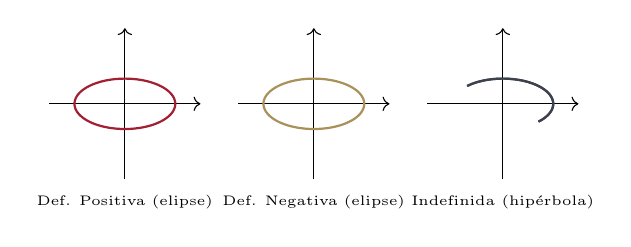
\begin{tikzpicture}[scale=0.8]
    % Definida positiva
    \begin{scope}
        \draw[->, thin] (-1.2,0) -- (1.2,0);
        \draw[->, thin] (0,-1.2) -- (0,1.2);
        \draw[MITCrimson, thick, domain=0:360, samples=100, smooth] 
            plot ({0.8*cos(\x)}, {0.4*sin(\x)});
        \node[below, font=\tiny] at (0,-1.3) {Def. Positiva (elipse)};
    \end{scope}
    
    % Definida negativa
    \begin{scope}[xshift=3cm]
        \draw[->, thin] (-1.2,0) -- (1.2,0);
        \draw[->, thin] (0,-1.2) -- (0,1.2);
        \draw[GoldLeaf, thick, domain=0:360, samples=100, smooth] 
            plot ({-0.8*cos(\x)}, {-0.4*sin(\x)});
        \node[below, font=\tiny] at (0,-1.3) {Def. Negativa (elipse)};
    \end{scope}
    
    % Indefinida
    \begin{scope}[xshift=6cm]
        \draw[->, thin] (-1.2,0) -- (1.2,0);
        \draw[->, thin] (0,-1.2) -- (0,1.2);
        \draw[SlateGrey, thick, domain=-45:135, samples=100, smooth] 
            plot ({0.8*cos(\x)}, {0.4*sin(\x)});
        \draw[SlateGrey, thick, domain=135:315, samples=100, smooth] 
            plot ({-0.8*cos(\x)}, {-0.4*sin(\x)});
        \node[below, font=\tiny] at (0,-1.3) {Indefinida (hipérbola)};
    \end{scope}
\end{tikzpicture}
\end{center}


\section{XXXIII. Formulación General}

\noindent\textbf{PROBLEMA DE PROGRAMACIÓN LINEAL (PL).} Encontrar $\mathbf{x} \in \mathbb{R}^n$ que:

\begin{equation}
\begin{aligned}
& \text{Maximizar} \quad z = \mathbf{c}^T\mathbf{x} \\
& \text{sujeto a} \quad \mathbf{Ax} \leq \mathbf{b} \\
& \quad \quad \quad \quad \mathbf{x} \geq \mathbf{0}
\end{aligned}
\end{equation}

\noindent\textbf{Componentes:}
\begin{itemize}
    \item $\mathbf{x}$: vector de variables de decisión
    \item $\mathbf{c}$: vector de coeficientes de la función objetivo
    \item $\mathbf{A}$: matriz de coeficientes tecnológicos
    \item $\mathbf{b}$: vector de recursos disponibles
\end{itemize}

\subsection{Formas Equivalentes}

\begin{voguebox}[title=Transformaciones Estándar]
\small
\begin{enumerate}
    \item \textbf{Minimización a maximización:} $\min \mathbf{c}^T\mathbf{x} = -\max (-\mathbf{c}^T\mathbf{x})$
    \item \textbf{Restricciones $\geq$ a $\leq$:} $\mathbf{Ax} \geq \mathbf{b} \Leftrightarrow -\mathbf{Ax} \leq -\mathbf{b}$
    \item \textbf{Restricciones de igualdad:} $\mathbf{Ax} = \mathbf{b} \Leftrightarrow \mathbf{Ax} \leq \mathbf{b}$ y $-\mathbf{Ax} \leq -\mathbf{b}$
\end{enumerate}
\end{voguebox}

\section{XXXIV. Formulación Matricial}

\noindent\textbf{EJEMPLO: Problema de Producción}

Una fábrica produce 2 productos usando 3 recursos:

\begin{align*}
\text{Max } z &= 40x_1 + 60x_2 \\
\text{s.a. } & 2x_1 + 4x_2 \leq 1000 \quad \text{(horas mano de obra)} \\
& 3x_1 + 2x_2 \leq 900 \quad \text{(horas máquina)} \\
& x_1 + x_2 \leq 300 \quad \text{(materia prima)} \\
& x_1, x_2 \geq 0
\end{align*}

\noindent\textbf{Forma Matricial:}

\begin{equation}
\mathbf{c} = \begin{bmatrix}40 \\ 60\end{bmatrix}, \quad
\mathbf{A} = \begin{bmatrix}2 & 4 \\ 3 & 2 \\ 1 & 1\end{bmatrix}, \quad
\mathbf{b} = \begin{bmatrix}1000 \\ 900 \\ 300\end{bmatrix}, \quad
\mathbf{x} = \begin{bmatrix}x_1 \\ x_2\end{bmatrix}
\end{equation}

\subsection{Representación Gráfica (para 2 variables)}

\begin{center}
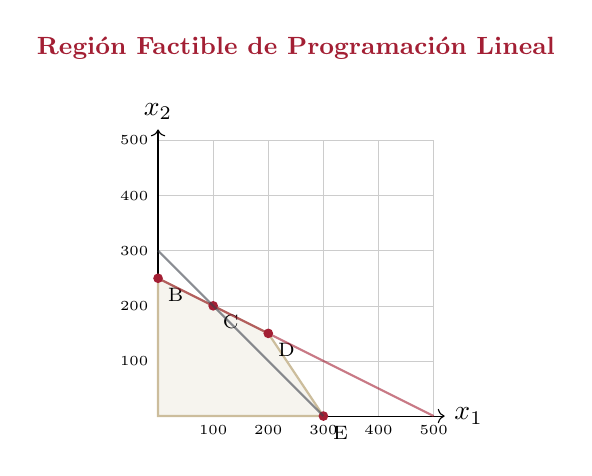
\begin{tikzpicture}[scale=0.7]
    % Marco y ejes simples
    \draw[gray!40, very thin] (0,0) grid (5,5);
    \draw[->] (0,0) -- (5.2,0) node[right] {$x_1$};
    \draw[->] (0,0) -- (0,5.2) node[above] {$x_2$};
    
    % REGIÓN FACTIBLE como elemento principal
    \fill[GoldLeaf!10, draw=GoldLeaf!60, thick] 
        (0,0) -- (0,2.5) -- (1,2) -- (2,1.5) -- (3,0) -- cycle;
    
    % Solo las intersecciones importantes
    \foreach \x/\y/\lab in {
        0/2.5/B,
        1/2/C,
        2/1.5/D,
        3/0/E
    } {
        \fill[MITCrimson] (\x,\y) circle (2.5pt);
        \node[font=\scriptsize, below right] at (\x,\y) {\lab};
    }
    
    % Líneas de restricción más sutiles
    \draw[MITCrimson, thick, opacity=0.6] (0,2.5) -- (5,0);
    \draw[SlateGrey, thick, opacity=0.6] (0,3) -- (3,0);
    
    % Etiquetas numéricas en ejes
    \foreach \x in {1,2,3,4,5}
        \node[below, font=\tiny] at (\x,0) {\x00};
    \foreach \y in {1,2,3,4,5}
        \node[left, font=\tiny] at (0,\y) {\y00};
        
    % Título claro
    \node[above, font=\small\bfseries, MITCrimson] at (2.5,6.3) 
        {Región Factible de Programación Lineal};
\end{tikzpicture}

{\footnotesize\textit{Nota: Las escalas representan cientos de unidades.}}
\end{center}



\section{XXXV. Conceptos Fundamentales}

\noindent\textbf{DEFINICIONES:}

\begin{definitionbox}[title=Solución Factible]
\small Un vector $\mathbf{x}$ que satisface todas las restricciones: $\mathbf{Ax} \leq \mathbf{b}$, $\mathbf{x} \geq \mathbf{0}$.
\end{definitionbox}

\begin{definitionbox}[title=Región Factible]
\small El conjunto de todas las soluciones factibles. En PL es un \textbf{poliedro convexo}.
\end{definitionbox}

\begin{definitionbox}[title=Solución Óptima]
\small Una solución factible que maximiza (o minimiza) la función objetivo.
\end{definitionbox}

\begin{definitionbox}[title=Punto Extremo (Vértice)]
\small Un punto de la región factible que no puede expresarse como combinación convexa de otros dos puntos distintos del conjunto.
\end{definitionbox}

\subsection{Teorema Fundamental de PL}

\begin{theorembox}[title=Existencia de Solución Óptima]
\small Si un problema de PL tiene solución óptima, entonces al menos un punto extremo de la región factible es solución óptima.
\end{theorembox}

\noindent\textbf{COROLARIO:} Para encontrar el óptimo, basta examinar los puntos extremos.

\section{XXXVI. Método Simplex (Conceptual)}

\noindent\textbf{IDEA FUNDAMENTAL:} Moverse de un punto extremo a otro adyacente mejorando la función objetivo, hasta alcanzar el óptimo.

\subsection{Forma Estándar}

Agregando variables de holgura $s_i \geq 0$:

\begin{equation}
\begin{aligned}
\text{Max } z &= 40x_1 + 60x_2 \\
\text{s.a. } & 2x_1 + 4x_2 + s_1 = 1000 \\
& 3x_1 + 2x_2 + s_2 = 900 \\
& x_1 + x_2 + s_3 = 300 \\
& x_1, x_2, s_1, s_2, s_3 \geq 0
\end{aligned}
\end{equation}

\noindent\textbf{Forma Matricial Ampliada:}

\begin{equation}
\begin{bmatrix}
2 & 4 & 1 & 0 & 0 \\
3 & 2 & 0 & 1 & 0 \\
1 & 1 & 0 & 0 & 1
\end{bmatrix}
\begin{bmatrix}
x_1 \\ x_2 \\ s_1 \\ s_2 \\ s_3
\end{bmatrix}
=
\begin{bmatrix}
1000 \\ 900 \\ 300
\end{bmatrix}
\end{equation}

\subsection{Tabla Simplex Inicial}

\begin{center}
\begin{tabular}{|c|ccccc|c|}
\hline
Base & $x_1$ & $x_2$ & $s_1$ & $s_2$ & $s_3$ & RHS \\
\hline
$s_1$ & 2 & 4 & 1 & 0 & 0 & 1000 \\
$s_2$ & 3 & 2 & 0 & 1 & 0 & 900 \\
$s_3$ & 1 & 1 & 0 & 0 & 1 & 300 \\
\hline
$z$ & -40 & -60 & 0 & 0 & 0 & 0 \\
\hline
\end{tabular}
\end{center}



\section{XXXVII. Análisis de Sensibilidad}

\noindent\textbf{PREGUNTAS CLAVE:}
\begin{enumerate}
    \item ¿Cómo cambia la solución si cambian los coeficientes $\mathbf{c}$?
    \item ¿Cómo cambia la solución si cambian los recursos $\mathbf{b}$?
    \item ¿Qué pasa si se agrega una nueva actividad (variable)?
\end{enumerate}

\subsection{1. Cambios en $\mathbf{c}$ (Coeficientes de la FO)}

\begin{voguebox}[title=Rango de Optimalidad]
\small Para cada variable no básica $x_j$, existe un intervalo $[c_j^-, c_j^+]$ tal que si $c_j$ permanece en ese intervalo, la base óptima no cambia.
\end{voguebox}

\noindent\textbf{EJEMPLO:} Para $x_2$ con $c_2 = 60$ en el problema anterior, podría encontrarse que el rango de optimalidad es $[40, 80]$.

\subsection{2. Cambios en $\mathbf{b}$ (Recursos)}

\begin{voguebox}[title=Rango de Factibilidad]
\small Para cada recurso $b_i$, existe un intervalo $[b_i^-, b_i^+]$ tal que si $b_i$ permanece en ese intervalo, las variables básicas óptimas no cambian (aunque sus valores sí).
\end{voguebox}

\noindent\textbf{EJEMPLO:} Para el primer recurso (1000 horas), podría encontrarse que el rango es $[800, 1200]$.

\subsection{3. Precios Sombra}

\begin{definitionbox}[title=Precio Sombra (Dual)]
\small El precio sombra $y_i$ del recurso $i$ es la tasa de cambio del valor óptimo $z^*$ con respecto a $b_i$:
\begin{equation}
y_i = \frac{\partial z^*}{\partial b_i}
\end{equation}
\end{definitionbox}

\noindent\textbf{Interpretación económica:} Valor marginal del recurso $i$.

\noindent\textbf{EJEMPLO:} Si $y_1 = 15$, significa que por cada hora adicional de mano de obra (recurso 1), la ganancia aumenta en \$15.

\section{XXXVIII. Dualidad en PL}

\noindent\textbf{PROBLEMA DUAL.} Asociado a cada problema de PL (primal) existe un problema dual:

\begin{center}
\begin{tabular}{|c|c|}
\hline
\textbf{Primal (Maximización)} & \textbf{Dual (Minimización)} \\
\hline
$\max \mathbf{c}^T\mathbf{x}$ & $\min \mathbf{b}^T\mathbf{y}$ \\
$\mathbf{Ax} \leq \mathbf{b}$ & $\mathbf{A}^T\mathbf{y} \geq \mathbf{c}$ \\
$\mathbf{x} \geq \mathbf{0}$ & $\mathbf{y} \geq \mathbf{0}$ \\
\hline
\end{tabular}
\end{center}

\noindent\textbf{TEOREMA DE DUALIDAD DÉBIL:} Para cualquier $\mathbf{x}$ factible primal y $\mathbf{y}$ factible dual:
\begin{equation}
\mathbf{c}^T\mathbf{x} \leq \mathbf{b}^T\mathbf{y}
\end{equation}

\noindent\textbf{TEOREMA DE DUALIDAD FUERTE:} Si el primal tiene solución óptima $\mathbf{x}^*$, entonces el dual tiene solución óptima $\mathbf{y}^*$ y:
\begin{equation}
\mathbf{c}^T\mathbf{x}^* = \mathbf{b}^T\mathbf{y}^*
\end{equation}



\section{XXXIX. Modelo de Leontief Generalizado}

\noindent\textbf{FORMULACIÓN DINÁMICA.} Extensión del modelo input-output a múltiples periodos:

\begin{equation}
\mathbf{x}_t = \mathbf{Ax}_t + \mathbf{B}(\mathbf{x}_{t+1} - \mathbf{x}_t) + \mathbf{d}_t
\end{equation}

donde:
\begin{itemize}
    \item $\mathbf{A}$: matriz de coeficientes de insumos corrientes
    \item $\mathbf{B}$: matriz de coeficientes de capital
    \item $\mathbf{d}_t$: demanda final en periodo $t$
\end{itemize}

\noindent\textbf{SOLUCIÓN:}
\begin{equation}
\mathbf{x}_t = (\mathbf{I} - \mathbf{A} + \mathbf{B})^{-1}(\mathbf{Bx}_{t+1} + \mathbf{d}_t)
\end{equation}

\subsection{Condición de Productividad}

\begin{theorembox}[title=Teorema de Hawkins-Simon Dinámico]
\small Para que exista una trayectoria de producción no negativa que satisfaga demandas finales no negativas, es necesario y suficiente que:
\begin{equation}
\det(\mathbf{I} - \mathbf{A} + \rho\mathbf{B}) > 0 \quad \forall \rho \in [0, 1]
\end{equation}
\end{theorembox}

\section{XL. Modelos de Equilibrio General}

\noindent\textbf{ECONOMÍA DE $n$ BIENES Y $m$ CONSUMIDORES.}

Cada consumidor $i$ tiene:
\begin{itemize}
    \item Dotación inicial: $\mathbf{w}_i \in \mathbb{R}^n$
    \item Función de utilidad: $u_i(\mathbf{x}_i)$
    \item Demanda: $\mathbf{x}_i(\mathbf{p})$ que maximiza utilidad sujeto a $\mathbf{p}^T\mathbf{x}_i \leq \mathbf{p}^T\mathbf{w}_i$
\end{itemize}

\noindent\textbf{CONDICIONES DE EQUILIBRIO:}

\begin{enumerate}
    \item \textbf{Maximización:} $\mathbf{x}_i(\mathbf{p})$ maximiza $u_i(\mathbf{x}_i)$ sujeto a restricción presupuestaria
    \item \textbf{Factibilidad:} $\sum_{i=1}^m \mathbf{x}_i(\mathbf{p}) \leq \sum_{i=1}^m \mathbf{w}_i$
    \item \textbf{Ley de Walras:} $\mathbf{p}^T\left(\sum_{i=1}^m \mathbf{x}_i(\mathbf{p}) - \sum_{i=1}^m \mathbf{w}_i\right) = 0$
\end{enumerate}

\subsection{Sistema de Ecuaciones}

\begin{equation}
\mathbf{F}(\mathbf{p}) = \sum_{i=1}^m \mathbf{x}_i(\mathbf{p}) - \sum_{i=1}^m \mathbf{w}_i = \mathbf{0}
\end{equation}

Dado que solo se determinan precios relativos, se normaliza $\sum_{j=1}^n p_j = 1$.



\section{XLI. Análisis de Estabilidad}

\noindent\textbf{SISTEMA DINÁMICO DE PRECIOS.} Modelo de ajuste walrasiano:

\begin{equation}
\frac{dp_j}{dt} = k_j \left(\sum_{i=1}^m x_{ij}(\mathbf{p}) - \sum_{i=1}^m w_{ij}\right), \quad j = 1,\ldots,n
\end{equation}

\noindent\textbf{LINEALIZACIÓN EN EL EQUILIBRIO $\mathbf{p}^*$:}

\begin{equation}
\frac{d\mathbf{p}}{dt} = \mathbf{J}(\mathbf{p}^*)(\mathbf{p} - \mathbf{p}^*)
\end{equation}

donde $\mathbf{J}(\mathbf{p}^*)$ es la matriz jacobiana de $\mathbf{F}$ en $\mathbf{p}^*$.

\subsection{Condición de Estabilidad}

\begin{theorembox}[title=Estabilidad de Lyapunov]
\small El equilibrio $\mathbf{p}^*$ es localmente estable si todos los valores propios de $\mathbf{J}(\mathbf{p}^*)$ tienen parte real negativa.
\end{theorembox}

\noindent\textbf{PROPIEDADES DE $\mathbf{J}$:}

\begin{enumerate}
    \item Homogeneidad de grado 0 en precios $\Rightarrow \mathbf{Jp} = \mathbf{0}$
    \item Ley de Walras $\Rightarrow$ suma de filas = 0
    \item En competencia perfecta con preferencias regulares, $\mathbf{J}$ tiene $n-1$ valores propios con parte real negativa
\end{enumerate}

\section{XLII. Modelos de Optimización Dinámica}

\noindent\textbf{PROBLEMA DE CONTROL ÓPTIMO.} Encontrar $\mathbf{u}(t)$ que:

\begin{equation}
\begin{aligned}
& \max \int_0^T f(t, \mathbf{x}(t), \mathbf{u}(t)) dt \\
& \text{sujeto a} \quad \frac{d\mathbf{x}}{dt} = \mathbf{g}(t, \mathbf{x}(t), \mathbf{u}(t)) \\
& \quad \quad \quad \quad \mathbf{x}(0) = \mathbf{x}_0, \quad \mathbf{x}(T) \geq \mathbf{0}
\end{aligned}
\end{equation}

\subsection{Condiciones de Pontryagin}

Definimos el hamiltoniano:
\begin{equation}
H(t, \mathbf{x}, \mathbf{u}, \mathbf{\lambda}) = f(t, \mathbf{x}, \mathbf{u}) + \mathbf{\lambda}^T\mathbf{g}(t, \mathbf{x}, \mathbf{u})
\end{equation}

Condiciones necesarias:
\begin{align}
\frac{\partial H}{\partial \mathbf{u}} &= \mathbf{0} \\
\frac{d\mathbf{\lambda}}{dt} &= -\frac{\partial H}{\partial \mathbf{x}} \\
\frac{d\mathbf{x}}{dt} &= \frac{\partial H}{\partial \mathbf{\lambda}}
\end{align}



\section{XLIII. Aplicación: Modelo de Crecimiento Óptimo}

\noindent\textbf{PROBLEMA DE RAMSEY-CASS-KOOPMANS.}

\begin{equation}
\begin{aligned}
& \max \int_0^\infty e^{-\rho t} u(c(t)) dt \\
& \text{sujeto a} \quad \frac{dk}{dt} = f(k(t)) - c(t) - \delta k(t) \\
& \quad \quad \quad \quad k(0) = k_0
\end{aligned}
\end{equation}

\noindent\textbf{HAMILTONIANO:}
\begin{equation}
H = e^{-\rho t} u(c) + \lambda[f(k) - c - \delta k]
\end{equation}

\noindent\textbf{CONDICIONES:}
\begin{align}
\frac{\partial H}{\partial c} &= e^{-\rho t} u'(c) - \lambda = 0 \\
\frac{d\lambda}{dt} &= -\frac{\partial H}{\partial k} = -\lambda[f'(k) - \delta] \\
\frac{dk}{dt} &= f(k) - c - \delta k
\end{align}

\subsection{Estado Estacionario}

En estado estacionario $\frac{dk}{dt} = \frac{dc}{dt} = 0$:

\begin{equation}
f'(k^*) = \rho + \delta, \quad c^* = f(k^*) - \delta k^*
\end{equation}

\section{XLIV. Econometría Matricial}

\noindent\textbf{MODELO DE REGRESIÓN LINEAL MÚLTIPLE.}

\begin{equation}
\mathbf{y} = \mathbf{X}\mathbf{\beta} + \mathbf{\varepsilon}
\end{equation}

donde:
\begin{itemize}
    \item $\mathbf{y}_{n \times 1}$: vector de observaciones de la variable dependiente
    \item $\mathbf{X}_{n \times k}$: matriz de variables independientes
    \item $\mathbf{\beta}_{k \times 1}$: vector de parámetros
    \item $\mathbf{\varepsilon}_{n \times 1}$: vector de errores
\end{itemize}

\noindent\textbf{ESTIMADOR MCO:}

\begin{equation}
\hat{\mathbf{\beta}} = (\mathbf{X}^T\mathbf{X})^{-1}\mathbf{X}^T\mathbf{y}
\end{equation}

\subsection{Propiedades}

\begin{enumerate}
    \item Insesgamiento: $E[\hat{\mathbf{\beta}}] = \mathbf{\beta}$ si $E[\mathbf{\varepsilon}] = \mathbf{0}$
    \item Matriz de varianzas-covarianzas: $\text{Var}(\hat{\mathbf{\beta}}) = \sigma^2 (\mathbf{X}^T\mathbf{X})^{-1}$
    \item Teorema de Gauss-Markov: Bajo condiciones estándar, $\hat{\mathbf{\beta}}$ es BLUE (Best Linear Unbiased Estimator)
\end{enumerate}

\noindent\textbf{COEFICIENTE DE DETERMINACIÓN:}

\begin{equation}
R^2 = 1 - \frac{\mathbf{e}^T\mathbf{e}}{\mathbf{y}^T\mathbf{y} - n\bar{y}^2}
\end{equation}

donde $\mathbf{e} = \mathbf{y} - \mathbf{X}\hat{\mathbf{\beta}}$ son los residuos.
\secbar

\section{XLV. Resumen de Conceptos Clave}

\noindent\textbf{1. ÁLGEBRA MATRICIAL BÁSICA}

\begin{itemize}
    \item \textbf{Matrices:} Arreglos rectangulares para sistemas de ecuaciones
    \item \textbf{Operaciones:} Suma, multiplicación escalar, multiplicación matricial (no conmutativa)
    \item \textbf{Transpuesta:} $(\mathbf{AB})^T = \mathbf{B}^T\mathbf{A}^T$
    \item \textbf{Inversa:} $\mathbf{A}^{-1}$ existe si $\det(\mathbf{A}) \neq 0$, $(\mathbf{AB})^{-1} = \mathbf{B}^{-1}\mathbf{A}^{-1}$
\end{itemize}

\noindent\textbf{2. SISTEMAS DE ECUACIONES}

\begin{itemize}
    \item \textbf{Forma matricial:} $\mathbf{Ax} = \mathbf{d}$
    \item \textbf{Solución:} $\mathbf{x} = \mathbf{A}^{-1}\mathbf{d}$ si $\mathbf{A}$ es no singular
    \item \textbf{Regla de Cramer:} $x_j = |\mathbf{A}_j|/|\mathbf{A}|$
    \item \textbf{Rango:} Número de ecuaciones independientes
\end{itemize}

\noindent\textbf{3. DETERMINANTES}

\begin{itemize}
    \item \textbf{Interpretación:} Volumen, criterio de invertibilidad
    \item \textbf{Propiedades:} Multiplicativo, dependencia lineal
    \item \textbf{Expansión:} Por cofactores
\end{itemize}

\noindent\textbf{4. VALORES Y VECTORES PROPIOS}

\begin{itemize}
    \item \textbf{Ecuación:} $\mathbf{Av} = \lambda\mathbf{v}$
    \item \textbf{Diagonalización:} $\mathbf{A} = \mathbf{PDP}^{-1}$
    \item \textbf{Aplicaciones:} Sistemas dinámicos, análisis de estabilidad
\end{itemize}

\noindent\textbf{5. FORMAS CUADRÁTICAS}

\begin{itemize}
    \item \textbf{Forma:} $Q(\mathbf{x}) = \mathbf{x}^T\mathbf{Ax}$, $\mathbf{A}$ simétrica
    \item \textbf{Clasificación:} Def. positiva, negativa, indefinida
    \item \textbf{Criterios:} Valores propios, menores principales
\end{itemize}

\noindent\textbf{6. PROGRAMACIÓN LINEAL}

\begin{itemize}
    \item \textbf{Formulación:} $\max \mathbf{c}^T\mathbf{x}$ s.a. $\mathbf{Ax} \leq \mathbf{b}$, $\mathbf{x} \geq \mathbf{0}$
    \item \textbf{Solución:} Método simplex, puntos extremos
    \item \textbf{Dualidad:} Problema dual, precios sombra
\end{itemize}

\section{XLVI. Referencias Bibliográficas}

\noindent\textbf{TEXTOS FUNDAMENTALES:}

\begin{enumerate}
    \item \textbf{Chiang, A. C. \& Wainwright, K.} (2005). \textit{Mathematical Economics}. McGraw-Hill.
    \item \textbf{Simon, C. P. \& Blume, L.} (1994). \textit{Mathematics for Economists}. Norton.
    \item \textbf{Sydsæter, K., Hammond, P., Seierstad, A., \& Strøm, A.} (2008). \textit{Further Mathematics for Economic Analysis}. Pearson.
    \item \textbf{Intriligator, M. D.} (2002). \textit{Mathematical Optimization and Economic Theory}. SIAM.
\end{enumerate}

\noindent\textbf{TEXTOS AVANZADOS:}

\begin{enumerate}
    \item \textbf{Luenberger, D. G.} (1995). \textit{Microeconomic Theory}. McGraw-Hill.
    \item \textbf{Mas-Colell, A., Whinston, M. D., \& Green, J. R.} (1995). \textit{Microeconomic Theory}. Oxford University Press.
    \item \textbf{Takayama, A.} (1985). \textit{Mathematical Economics}. Cambridge University Press.
\end{enumerate}

\noindent\textbf{ÁLGEBRA LINEAL:}

\begin{enumerate}
    \item \textbf{Strang, G.} (2016). \textit{Introduction to Linear Algebra}. Wellesley-Cambridge Press.
    \item \textbf{Lax, P. D.} (2007). \textit{Linear Algebra and Its Applications}. Wiley.
    \item \textbf{Meyer, C. D.} (2000). \textit{Matrix Analysis and Applied Linear Algebra}. SIAM.
\end{enumerate}



\section{XLVII. Problemas Representativos}

\noindent\textbf{PROBLEMA 1: Sistema de Mercado}

Dado el modelo de mercado:
\begin{align*}
Q_d &= 100 - 2P + 0.1Y \\
Q_s &= -20 + 3P \\
Y &= 500
\end{align*}

Encontrar el equilibrio $(P^*, Q^*)$ usando álgebra matricial.

\noindent\textbf{SOLUCIÓN:}
\begin{equation}
\begin{split}
\begin{bmatrix}
1 & 2 \\
1 & -3
\end{bmatrix}
\begin{bmatrix}
Q \\ P
\end{bmatrix}
&=
\begin{bmatrix}
150 \\ -20 
\end{bmatrix}\\
&\quad \Rightarrow \quad
\begin{bmatrix}
Q \\ P
\end{bmatrix}
=
\frac{1}{-5}
\begin{bmatrix}
-3 & -2 \\
-1 & 1
\end{bmatrix}
\begin{bmatrix}
150 \\ -20
\end{bmatrix} 
= \begin{bmatrix}
82 \\ 34
\end{bmatrix}
\end{split}
\end{equation}





\noindent\textbf{PROBLEMA 2: Determinante y Rango}

Determinar el rango de:
\begin{equation}
\mathbf{A} = \begin{bmatrix}
1 & 2 & 3 \\
2 & 4 & 6 \\
3 & 6 & 9
\end{bmatrix}
\end{equation}

\noindent\textbf{SOLUCIÓN:} Todas las filas son proporcionales, $\det(\mathbf{A}) = 0$, rango$(\mathbf{A}) = 1$.

\noindent\textbf{PROBLEMA 3: Valores Propios}

Encontrar valores y vectores propios de:
\begin{equation}
\mathbf{B} = \begin{bmatrix}
4 & 1 \\
2 & 3
\end{bmatrix}
\end{equation}

\noindent\textbf{SOLUCIÓN:}
$\lambda_1 = 2$, $\mathbf{v}_1 = \begin{bmatrix}1 \\ -2\end{bmatrix}$;
$\lambda_2 = 5$, $\mathbf{v}_2 = \begin{bmatrix}1 \\ 1\end{bmatrix}$

\vspace{0.5cm}
\noindent\textbf{PROBLEMA 4: Forma Cuadrática}

Clasificar $Q(x,y) = 2x^2 + 4xy + 5y^2$

\noindent\textbf{SOLUCIÓN:}
\begin{equation}
\mathbf{A} = \begin{bmatrix}2 & 2 \\ 2 & 5\end{bmatrix}, \quad
D_1 = 2 > 0, \quad D_2 = 10 - 4 = 6 > 0
\end{equation}
$\Rightarrow$ definida positiva.

\section{XLVIII. Software y Herramientas}

\noindent\textbf{PAQUETES DE SOFTWARE:}

\begin{itemize}
    \item \textbf{MATLAB:} Estándar industrial para álgebra matricial
    \item \textbf{Python:} NumPy, SciPy, pandas para análisis económico
    \item \textbf{R:} Especializado en estadística y econometría
    \item \textbf{Julia:} Alto desempeño para computación científica
    \item \textbf{Mathematica:} Cálculo simbólico y numérico
\end{itemize}

\noindent\textbf{LIBRERÍAS ESPECÍFICAS:}

\begin{itemize}
    \item \textbf{Optimización:} CVXOPT (Python), Optim (Julia)
    \item \textbf{Econometría:} statsmodels (Python), econometrics (R)
    \item \textbf{Álgebra lineal:} LAPACK, BLAS (subrutinas fundamentales)
\end{itemize}



\section{XLIX. Glosario de Términos}

\begin{tabularx}{\columnwidth}{p{0.4\columnwidth} p{0.5\columnwidth}}
\toprule
\textbf{Término} & \textbf{Definición} \\
\midrule
Matriz no singular & $\det(\mathbf{A}) \neq 0$, tiene inversa \\
Matriz singular & $\det(\mathbf{A}) = 0$, no tiene inversa \\
Rango & Número máximo de filas/columnas independientes \\
Traza & Suma de elementos diagonales: $\text{tr}(\mathbf{A}) = \sum a_{ii}$ \\
Determinante & Escalar que indica invertibilidad y volumen \\
Valor propio & $\lambda$ tal que $\mathbf{Av} = \lambda\mathbf{v}$ \\
Vector propio & $\mathbf{v} \neq \mathbf{0}$ tal que $\mathbf{Av} = \lambda\mathbf{v}$ \\
Diagonalización & $\mathbf{A} = \mathbf{PDP}^{-1}$ con $\mathbf{D}$ diagonal \\
Forma cuadrática & $Q(\mathbf{x}) = \mathbf{x}^T\mathbf{Ax}$, $\mathbf{A}$ simétrica \\
Definida positiva & $Q(\mathbf{x}) > 0$ para todo $\mathbf{x} \neq \mathbf{0}$ \\
Programación lineal & Optimización lineal con restricciones lineales \\
Región factible & Conjunto de puntos que satisfacen todas las restricciones \\
Punto extremo & Vértice de la región factible poliedral \\
Método simplex & Algoritmo para resolver problemas de PL \\
Problema dual & Problema de PL asociado al primal \\
Precio sombra & Tasa de cambio del valor óptimo respecto a un recurso \\
Modelo de Leontief & $\mathbf{x} = \mathbf{Ax} + \mathbf{d}$, economía input-output \\
Equilibrio general & Sistema de precios que vacía todos los mercados \\
\bottomrule
\end{tabularx}

\section{L. Consejos de Estudio}

\noindent\textbf{ESTRATEGIAS EFECTIVAS:}

\begin{enumerate}
    \item \textbf{Practicar con ejemplos pequeños:} Dominar casos 2×2 y 3×3 antes de generalizar
    \item \textbf{Visualizar:} Usar interpretaciones geométricas siempre que sea posible
    \item \textbf{Conectar conceptos:} Relacionar álgebra matricial con aplicaciones económicas
    \item \textbf{Verificar propiedades:} Comprobar teoremas con ejemplos numéricos
    \item \textbf{Usar software:} Implementar algoritmos para comprenderlos mejor
\end{enumerate}

\noindent\textbf{ERRORES COMUNES:}

\begin{itemize}
    \item Asumir conmutatividad en multiplicación de matrices
    \item Confundir $\mathbf{AB}$ con $\mathbf{BA}$
    \item Olvidar verificar condiciones para invertir matrices
    \item No considerar restricciones de dimensionalidad
    \item Ignorar interpretaciones económicas de resultados matemáticos
\end{itemize}

\subsection{Mensaje Final}

\begin{voguebox}[title=La Elegancia del Álgebra Matricial]
\small El álgebra de matrices no es solo una herramienta computacional; es un lenguaje que revela la estructura profunda de los modelos económicos. Su poder reside en la capacidad de tratar sistemas complejos de manera unificada, transformando problemas aparentemente intratables en formulaciones elegantes y resolubles.
\end{voguebox}

\secbar

\begin{voguebox}[title=Contacto \& Referencias]
\centering
\vspace{6pt}

% Encabezado con nombre y título
{\Large\textbf{\textcolor{MITCrimson}{Emanuel Quintana Silva}}}\\[2pt]
{\small\textit{Economista en formación · UPTC · he/him}}\\[6pt]

% Descripción
\noindent\begin{minipage}{0.95\textwidth}
\centering\footnotesize
Economista en formación con gran pasión por la Econometría Computacional y la aplicación de R y Python en la Estadística y las Ciencias Sociales.
\end{minipage}

\vspace{10pt}

% Línea divisoria decorativa
\rule{0.8\textwidth}{0.2pt}

\vspace{1pt}

% Información de contacto en dos columnas mejor espaciadas
\noindent\begin{minipage}[t]{0.49\textwidth}
\raggedright\footnotesize
\textbf{\hspace{2pt}Email:}\\[2pt]
{\small emanuel.quintana@uptc.edu.co}

\vspace{8pt}

\textbf{\hspace{2pt}ORCID:}\\[2pt]
\href{https://orcid.org/0009-0006-8419-2805}{\small 0009-0006-8419-2805}
\end{minipage}

\vspace{14pt}

% Línea divisoria
\rule{0.8\textwidth}{0.2pt}

\vspace{14pt}

\textbf{ \hspace{4pt}GitHub:}\\[2pt]
\href{https://github.com/emanuelquintana-glitch} {\small emanuelquintana-glitch}


\vspace{8pt}

\textbf{\hspace{2pt}Repositorio:}\\[2pt]
\small\url{https://github.com/emanuelquintana-glitch/-Apuntes_Economia_Matematica.git}

\vspace{8pt}

% Estadísticas centradas
{\footnotesize 
\faIcon{users} \textbf{3} seguidores · 
\faIcon{user-friends} \textbf{78} siguiendo · 
\faIcon{database} Repositorio activo
}

\vspace{5pt}
\end{voguebox}


\end{multicols*}

\begin{tikzpicture}[remember picture, overlay]
    \draw[VogueBlack, line width=0.5pt] ($(current page.south west) + (0.5in, 0.4in)$) -- ($(current page.south east) + (-0.5in, 0.4in)$);
    \node[anchor=west] at ($(current page.south west) + (0.5in, 0.25in)$) {\tiny \textcopyright\ 2025 Emanuel Quintana Silva \textbar\ UPTC \textbar\ Economía Matemática \textbar\ Todos los derechos reservados};
    \node[anchor=east] at ($(current page.south east) + (-0.5in, 0.25in)$) {\tiny \texttt{Última actualización: Diciembre 2025}};
\end{tikzpicture}



\end{document}